%%
%% This is file `sample-sigconf.tex',
%% generated with the docstrip utility.
%%
%% The original source files were:
%%
%% samples.dtx  (with options: `sigconf')
%% 
%% IMPORTANT NOTICE:
%% 
%% For the copyright see the source file.
%% 
%% Any modified versions of this file must be renamed
%% with new filenames distinct from sample-sigconf.tex.
%% 
%% For distribution of the original source see the terms
%% for copying and modification in the file samples.dtx.
%% 
%% This generated file may be distributed as long as the
%% original source files, as listed above, are part of the
%% same distribution. (The sources need not necessarily be
%% in the same archive or directory.)
%%
%%
%% Commands for TeXCount
%TC:macro \cite [option:text,text]
%TC:macro \citep [option:text,text]
%TC:macro \citet [option:text,text]
%TC:envir table 0 1
%TC:envir table* 0 1
%TC:envir tabular [ignore] word
%TC:envir displaymath 0 word
%TC:envir math 0 word
%TC:envir comment 0 0
%%
%%
%% The first command in your LaTeX source must be the \documentclass command.
\documentclass[sigconf]{acmart}


\usepackage{xcolor}
\usepackage{booktabs}
\usepackage{multirow}
%\usepackage[english]{babel}
%\usepackage{environ}
%\usepackage{newclude}
%\usepackage{rotating}
%\usepackage{pdflscape}
\usepackage{adjustbox}
%%% Pseudocodes
%\usepackage{inconsolata}
%\usepackage{floatrow}
%\newfloatcommand{capbtabbox}{table}[][\FBwidth]
\usepackage{graphicx}
\usepackage{caption}
%\usepackage{subcaption}

\usepackage{tabularx}% added for table design
\usepackage[noend]{algpseudocode}
%% Multiline
\newcommand\CONDITION[2]%
{\begin{tabular}[t]{@{}l@{}l@{}}
		#1&#2
	\end{tabular}%
}
\algdef{SE}[WHILE]{While}{EndWhile}[1]%
{\algorithmicwhile\ \CONDITION{#1}{\ \algorithmicdo}}%
{\algorithmicend\ \algorithmicwhile}
\algdef{SE}[FOR]{For}{EndFor}[1]%
{\algorithmicfor\ \CONDITION{#1}{\ \algorithmicdo}}%
{\algorithmicend\ \algorithmicfor}
\algdef{S}[FOR]{ForAll}[1]%
{\algorithmicforall\ \CONDITION{#1}{\ \algorithmicdo}}
\algdef{SE}[REPEAT]{Repeat}{Until}{\algorithmicrepeat}[1]%
{\algorithmicuntil\ \CONDITION{#1}{}}
\algdef{SE}[IF]{If}{EndIf}[1]%
{\algorithmicif\ \CONDITION{#1}{\ \algorithmicthen}}%
{\algorithmicend\ \algorithmicif}%
\algdef{C}[IF]{IF}{ElsIf}[1]%
{\algorithmicelse\ \algorithmicif\ \CONDITION{#1}{\ \algorithmicthen}}
%% End Multiline
\usepackage{algorithm,algorithmicx}
%\makeatletter
%\algrenewcommand\ALG@beginalgorithmic{\ttfamily}
%\makeatother
\usepackage{adjustbox} %% Fitting to pageRichard
\usepackage{amsmath,stmaryrd}
%% mathematics
\usepackage{braket} %% Set, tuple...
\usepackage{pifont,bigdelim}
\usepackage{amsmath,amssymb}
\newcommand{\Next}{\ensuremath{\mathbf{X}}}
\newcommand{\Globally}{\ensuremath{\mathbf{G}}}
\newcommand{\Future}{\ensuremath{\mathbf{F}}}
\newcommand{\WeakUntil}[2]{\ensuremath{{#1}\;\mathbf{W}\;{#2}}}
\newcommand{\DUntil}[2]{\ensuremath{{#1}\;\mathbf{U}\;{#2}}}
\newcommand{\MonoDeclareClause}[4]{\textsf{#1}(\texttt{#2},#3,{#4})}
\newcommand{\DeclareClause}[5]{\textsf{#1}(\texttt{#2},#3,\texttt{#4},#5)}
\newcommand{\DeclareClauseWithJoin}[6]{\textsf{#1}(\texttt{#2},#3,\texttt{#4},#5)\;\textsf{where}\;#6}
\newcommand{\Sdeclare}[3]{\DeclareClause{#1}{#2}{\textbf{true}}{#3}{\textbf{true}}}
\newcommand{\LTLf}{\textup{LTL}\textsubscript{f}\;}

%%
%% \BibTeX command to typeset BibTeX logo in the docs
\AtBeginDocument{%
  \providecommand\BibTeX{{%
    Bib\TeX}}}

%% Rights management information.  This information is sent to you
%% when you complete the rights form.  These commands have SAMPLE
%% values in them; it is your responsibility as an author to replace
%% the commands and values with those provided to you when you
%% complete the rights form.
\setcopyright{acmcopyright}
\copyrightyear{2022}
\acmYear{2022}
\acmDOI{XXXXXXX.XXXXXXX}
%% These commands are for a PROCEEDINGS abstract or paper.
\acmConference[IDEAS'22]{26th International Database Application \& Enginnerring Symosium}{August 22--24,
  2022}{Budapest, HU}
\acmPrice{15.00}
\acmISBN{978-1-4503-XXXX-X/18/06}


%%
%% Submission ID.
%% Use this when submitting an article to a sponsored event. You'll
%% receive a unique submission ID from the organizers
%% of the event, and this ID should be used as the parameter to this command.
%%\acmSubmissionID{123-A56-BU3}

%%
%% For managing citations, it is recommended to use bibliography
%% files in BibTeX format.
%%
%% You can then either use BibTeX with the ACM-Reference-Format style,
%% or BibLaTeX with the acmnumeric or acmauthoryear sytles, that include
%% support for advanced citation of software artefact from the
%% biblatex-software package, also separately available on CTAN.
%%
%% Look at the sample-*-biblatex.tex files for templates showcasing
%% the biblatex styles.
%%

%%
%% The majority of ACM publications use numbered citations and
%% references.  The command \citestyle{authoryear} switches to the
%% "author year" style.
%%
%% If you are preparing content for an event
%% sponsored by ACM SIGGRAPH, you must use the "author year" style of
%% citations and references.
%% Uncommenting
%% the next command will enable that style.
%%\citestyle{acmauthoryear}



%%
%% end of the preamble, start of the body of the document source.
\begin{document}

%%
%% The "title" command has an optional parameter,
%% allowing the author to define a "short title" to be used in page headers.
	\title{Running Temporal Logical Queries on the Relational Model}

%%
%% The "author" command and its associated commands are used to define
%% the authors and their affiliations.
%% Of note is the shared affiliation of the first two authors, and the
%% "authornote" and "authornotemark" commands
%% used to denote shared contribution to the research.
\author{Samuel Appleby}
\orcid{0000-0003-2608-0881}
\email{s.appleby3@newcastle.ac.uk}
\affiliation{%
	\institution{Newcastle University\\ School of Computing}
	\country{United Kingdom}
}


\author{Giacomo Bergami}
\orcid{0000-0002-1844-0851}
\email{ngb113@newcastle.ac.uk}
\affiliation{%
	\institution{Newcastle University\\ School of Computing}
	\country{United Kingdom}
}


\author{Graham Morgan}
\orcid{0000-0002-0089-0395}
\email{graham.morgan@newcastle.ac.uk}
\affiliation{%
	\institution{Newcastle University\\ School of Computing}
	\country{United Kingdom}
}

%%
%% By default, the full list of authors will be used in the page
%% headers. Often, this list is too long, and will overlap
%% other information printed in the page headers. This command allows
%% the author to define a more concise list
%% of authors' names for this purpose.
	\renewcommand{\shortauthors}{Appleby et al.}

%%
%% The abstract is a short summary of the work to be presented in the
%% article.
\begin{abstract}
State of the art for model checking exploit computationally intensive solutions, bottlenecked by either repeated data access or suboptimal algorithmic implementations. Our solution outperforms the previous solutions while proposing novel temporal logic operators for accessing relational tables.	
\end{abstract}

%%
%% The code below is generated by the tool at http://dl.acm.org/ccs.cfm.
%% Please copy and paste the code instead of the example below.
%%
\begin{CCSXML}
<ccs2012>
 <concept>
  <concept_id>10010520.10010553.10010562</concept_id>
  <concept_desc>Computer systems organization~Embedded systems</concept_desc>
  <concept_significance>500</concept_significance>
 </concept>
 <concept>
  <concept_id>10010520.10010575.10010755</concept_id>
  <concept_desc>Computer systems organization~Redundancy</concept_desc>
  <concept_significance>300</concept_significance>
 </concept>
 <concept>
  <concept_id>10010520.10010553.10010554</concept_id>
  <concept_desc>Computer systems organization~Robotics</concept_desc>
  <concept_significance>100</concept_significance>
 </concept>
 <concept>
  <concept_id>10003033.10003083.10003095</concept_id>
  <concept_desc>Networks~Network reliability</concept_desc>
  <concept_significance>100</concept_significance>
 </concept>
</ccs2012>
\end{CCSXML}

\ccsdesc[500]{Computer systems organization~Embedded systems}
\ccsdesc[300]{Computer systems organization~Redundancy}
\ccsdesc{Computer systems organization~Robotics}
\ccsdesc[100]{Networks~Network reliability}

%%
%% Keywords. The author(s) should pick words that accurately describe
%% the work being presented. Separate the keywords with commas.
\keywords{Logical Artificial Intelligence, Knowledge Bases, Query Plan, Temporal Logic}
%% A "teaser" image appears between the author and affiliation
%% information and the body of the document, and typically spans the
%% page.
%\begin{teaserfigure}
%  \includegraphics[width=\textwidth]{sampleteaser}
%  \caption{Seattle Mariners at Spring Training, 2010.}
%  \Description{Enjoying the baseball game from the third-base
%  seats. Ichiro Suzuki preparing to bat.}
%  \label{fig:teaser}
%\end{teaserfigure}

%%
%% This command processes the author and affiliation and title
%% information and builds the first part of the formatted document.
\maketitle

\section{Introduction}

%\paragraph*{Brief introduction of your general area of interest: provide the \textbf{context} to the overall general setting.} 
\textit{Conformance checking} is an integral part of \textsc{Artificial Intelligence} {bridging} data mining and business process management \cite{bpm21}. It assesses whether a sequence of distinguishable events (i.e., a \textit{trace}) conforms to the expected process behaviour represented as a \textit{(process) model} \cite{RozinatA08}. Each event is associated with both an \textit{activity label} describing the captured event, as well as payload data, either associated to the whole trace or to a specific event. When multiple distinct traces are considered in a log, model checking lists the %set of
 traces satisfying the model \cite{BurattinMS16}. Non-conforming traces  are usually referred to as \textit{deviant} \cite{bpm21}.  \textit{Declarative} models are composed of multiple human-readable \textit{clauses} that should be  jointly satisfied (i.e., \textit{conjunctive query}) \cite{Li2020}; each of these is the instantiation of a specific behavioural pattern (i.e., \textit{template}) expressing temporal correlations between actions being carried out thus linking preconditions to expected outcomes. Such correlations might  also involve % extended with 
 %data conditions, thus expressing
  $\Theta$-joins between activated and targeted events. %only between their associated payload.  
 Models
 %with specific data and action conditions. These high level representations 
 can be %also 
 expressed as Finite State Machines \cite{MultiPerspective,AgostinelliBFMM21} %Such a model might be either represented as a set of temporal clauses, determining correlations between events happening at a previous time of the trace (\textit{activation}) and others happening in the immediate future (\textit{target}).
 but, by doing so, each state will represent a possible state configuration the system might find itself in, for which we need to describe all the reasonable actions and data conditions. %the system might find itself in. 
 This makes graph data-aware model checking as \cite{bpm21} rather inefficient, as the size of these graphs becomes exponential with respect to the original size of the declarative model. As a result, this increases the computational time required for conformance checking. Such models are also incapable of expressing $\Theta$-correlation conditions on the data payload, thus limiting the models' expressiveness.
 
\begin{figure*}
	\centering
	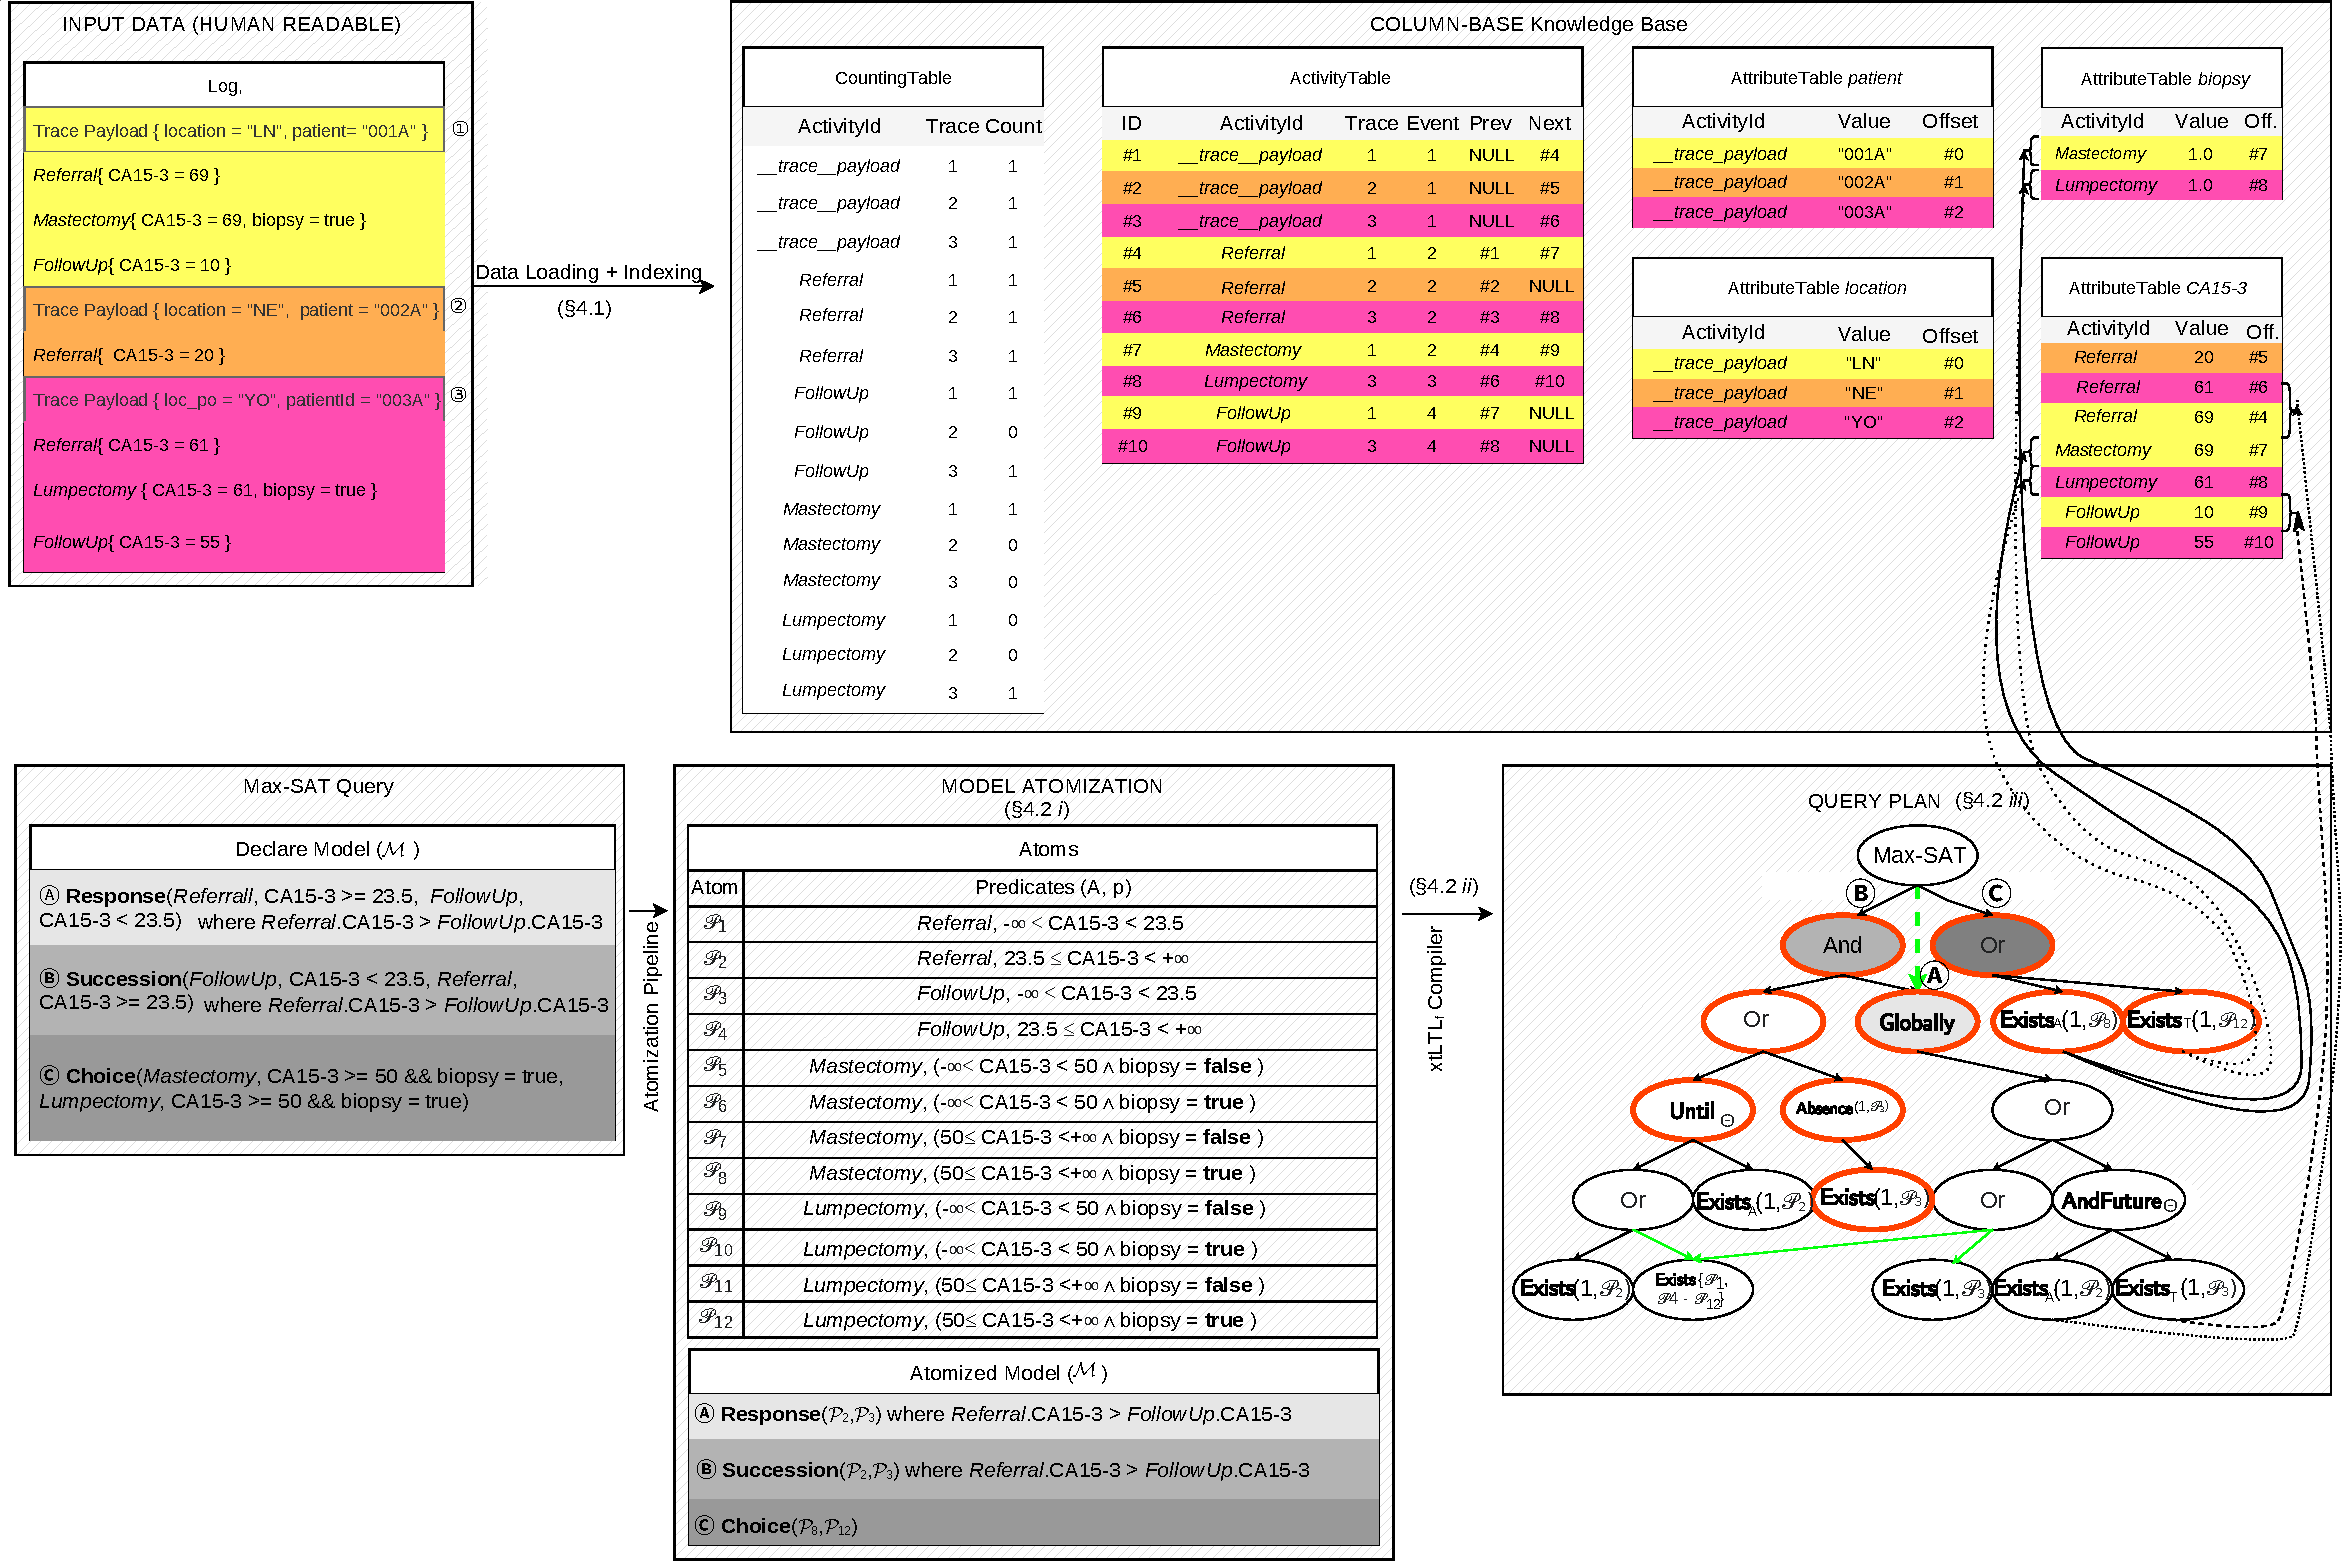
\includegraphics[width=\textwidth]{images/knobab_pipeline.pdf}
	\caption{KnoBAB Architecture for Breast Cancer patients. Each trace \ding{192}-\ding{194} represents one single patient's clinical history, are represented with unique colouring. Please observe that the atomization process does not consider data distribution but rather partitions the data space as described by the data activation and target conditions. In the query plan, green arrows remark access  to shared sub-queries as in \cite{BellatrecheKB21}, and thick red ellipses remark which operators are untimed. } \label{fig:knobab_pipeline}
\end{figure*}
Conformance checking with declarative models
%{Despite the two approaches are equivalent} , {the latter is rather inefficient for conformance checking traces with data payloads} \cite{bpm21}. %Declarative temporal rules are not limited to the mere presence of specific events within the trace, but also determine \RevRepl{how such clauses might occur}{temporal occurrence patterns}. 
{is a well-studied technology at the core} of AI's temporal decision making. \textit{Firstly}, conformance checking is adopted when mining a model from logs either containing only positive (or negative) traces \cite{ROVANI20159236}, or on logs containing both, but where positive traces can be discriminated from the negative ones via behavioural or data conditions, thus allowing to generate both a positive and a negative model  \cite{mining}. 
{The example proposed in this paper (\figurename~\ref{fig:knobab_pipeline}), contains cancer patient records obtained from a hospital (this data is included in our datasets\footnoteref{footnote:datasets}). In healthcare, individuals likely to suffer from an illness should receive treatment, and those that are not suffering should not. Therefore, cases where sufferers not receiving treatment (false negatives) and non-sufferers receiving treatment (false positives) needs to be minimised. \figurename~\ref{fig:knobab_pipeline} proposes a simplified scenario for defining this scenario. We conisder 2 event payload labels: \textsf{CA 15-3} (cancer antigen concentration in a patients blood), and \textsf{biopsy} (biopsies should be taken before any procedure is acted upon). Our model targets only breast cancer patients with successful therapies, that describes a medical protocol and the desired patients' health condition at each step. } %\remove{In a hospital scenario, a positive model might both describe a medical protocol and the desired patients' health condition at each step.} %these might identify the desired health conditions at the end of a medical protocol or simply state the viable solutions.
 %\remove{E.g., For the positive models  in  target only breast cancer patients with successful therapies:}  
 \Circled{\small C} {states} two possible surgical operations for  breast tumours  are  mastectomy or lumpectomy if the biopsy is positive and the CA-13.5 is way above ($\geq 50$) the guard level being 23.5 units per \textit{ml},  and   \Circled{\small A}-\Circled{\small B}  any successful treatment should decrease the CA-13.5 levels, which should be below the guard level; such correlation data condition is expressed via a $\Theta$ condition (also indicated as  \textsf{where}). A twinned negative model (not in \figurename) might better discriminate healthy patients from patients where the therapy was unsuccessful.
%by extracting a declarative model out of a hospital log  containing `successful' traces (e.g., correct procedures, adequate medication), we extract the temporal correlation conditions linking good pre-conditions to expected outcomes  \cite{Amantea2020}. 
\textit{Secondly}, conformance checking can also exploit such models
for predicting which novel clinical situations represented as %on the novel hospital 
traces are likely to adhere to the expected clinical standards. Novel situations can be represented as a log: e.g., in \figurename~\ref{fig:knobab_pipeline}, we have three patients: \ding{192} a cancer patient with a successful mastectomy, \ding{193} a healthy patient, and \ding{194} an unsuccessful lumpectomy, thus suggesting that the patient might still have some cancerous cells. Given the aforementioned model, patient \ding{192} will satisfy the model as the surgical operation was successful, \ding{193} will not satisfy the model because neither mastectomy nor lumpectomy was required {($\mathcal{M}$ is only fulfilled for \textit{successful} procedures)}, and \ding{194} will not satisfy the  target condition, even though the correlation condition was met. Our model of interest should only return %\remove{the first patient}
 {\ding{192}} as an outcome of the conformance checking process.
% \RevRepl{this}{the resulting mined} model \RevRepl{for a current trace to provide the action}{for determining} which \RevAdd{clinical situation} is likely to \RevRepl{be  the next correct decision}{adhere to the expected clinical standards}.



%%\pdfcomment[author=Giacomo]{Please link this description to the infographics, that is going to describe the whole KnoBAB pipeline}
%When a trace does not adhere to the model, we say that the trace is \textit{deviant} \cite{bpm21}. %\RevDel{In the case of traces, the order of the events is important, and temporal information of each event must be stored.}
%E.g., Given a Declare template \textsf{Response}, \DeclareClause{Response}{A}{\textbf{true}}{B}{\textbf{true}} is the instantiated Declare \textit{clause} for \textit{activity labels} \texttt{A} and \texttt{B} stating ``\emph{If event \texttt{A}  happens, event \texttt{B}  must happen either contemporarily or anytime in the future}'' (\figurename~\ref{fig:comparison}); \texttt{A}  (\texttt{B}) is called  \textit{activation} (\textit{target}) condition; a trace would be a deviant \emph{iff.} a trace contained an instance of \texttt{A}  that was not followed by an instance of \texttt{B}. 
%In \figurename~\ref{fig:comparison}, the last trace is the only deviant one. Furthermore, \textbf{true} predicates associated to activation (target) conditions can be enriched to express data conditions (\S\ref{sec:DAD}). As any declarative language, the specification of such templates can be expressed as expressions of logical operators: in this field, Finite Liniear Time Logic (\LTLf) is usually exploited. For instance, clause $\DeclareClause{Precedence}{A}{p}{B}{q}$ becomes $\WeakUntil{\neg(\texttt{B} \wedge q)}{(\texttt{A} \wedge p)}$, %\pdfcomment[author=Giacomo]{Please link this description to the infographics, that is going to describe the whole KnoBAB pipeline} 
%where the binary operator $\WeakUntil{}{}$ denotes that either left-hand-side should always occur until the right- one is found for the first time in the trace, or the left-hand-side should always occur (\figurename~\ref{fig:comparison}). %Activation and target 
%%Conditions might %be 
%%also include % extended with 
%%\textit{correlation} conditions, thus expressing $\Theta$-joins between activated and targeted events. %only between their associated payload. 
%%This is a restriction over traditional relational algebra operators, as we are only interested in analysing such correspondence. %Figure \ref{fig:comparison} exemplifies such intuition.
%%%%{\color{red}[TODO: replace] To further decompose these clauses, algebraic notation can be used to represent the set of operators that are the constituents of a given clause. Declare templates can be represented using \LTLf \cite{Li2020}. This allows for a flexible conformance checking implementation, as each clause can be represented as a unique pairing of \LTLf operators and join operators, for insatnce $\mathbf{RespondedExistence(A,B)}$ becomes $\Future(A) \Rightarrow \Future(B)$\PopUpComment{Giacomo}{Please observe that mathcal should be used only by surrounding the symbol of interest. Otherwise, in some other scenarios, you might have faults. Still, we are going to use a box/diamond notation for this paper. I added some macros for that}. As part of the process mining pipeline, conformance checking is used to identify patterns emerging from a given log. Therefore, process mining can actually be reduced to a conformance checking problem.}\PopUpComment{Giacomo}{Some of the contents in here are good, and should be put elsewhere in the introduction. "In fact, despite these operators might be applied to query plans similarly to relational algebra operators, no work -- to the best of our knowledge -- exploited this possibility". But, this should be linked to another kind of problem, too!}



%\paragraph*{Why do I want to talk about this problem? Why is it relevant?} \textit{Because current literature is lacking of a given aspect} 
%\section{Motivating Example}\label{sec:mot}
%Correlations might be also exploited in 
Real business use case scenarios usually require $\Theta$-correlations. In a goods brokerage scenario \cite{PetermannJMR14},  items are traded between producers (vendors) and retailers (customers): each transaction starts with a vendor sending a sales quotation to a customer. If an offer is accepted and the order is confirmed, then the item is scheduled for delivery. When ready, a logistic operator collects it. %The 
%sales invoice and the sales order is then sent to the retailer. Next, both the producers and the retailers might rank the items on a scale from 0 to 10, where 0 denotes a despicable product while 10 denotes an excellent one. A retailer ranking a product extremely low can file a complaint ticket to the brokerage company which might grant a refund.
In this scenario, deviant traces %are %traces that 
either do not reflect the company's rules or %traces that 
will potentially lead to retailers' complaints: %In particular, a company must send a product only after receiving the offer's acceptance. \dfrac{num}{den}
e.g., % business rule explicitly requiring correlations is the following:   
a late delivery complaint can occur only if the date the product is received is greater than the agreed time to receive it as registered in a previous agreement event. This situation cannot be directly expressed as a temporal pattern, as we also need to test the timestamps associated in the data payload. %Albeit this task requires to represent temporal information within the data perspective \cite{MultiPerspective}, this would require to express \textit{correlation} conditions (\S\ref{sec:DAD}) within the single Declare template of interest. 
%
%\paragraph*{Who might be interested in our solution? How these people might use this work?} \textit{Please provide the pieces of information that are specific to your own research field, and provide some use case examples motivating the practicality of your approach}  
%
{Conformance checking can be applied to several unexplored non-business domains, such as smart contract verification \cite{10.1007/978-3-031-08421-8_9}.} 
% \textit{First}, given that process model information can be exploited to represent 
%  tasks performed by both physical and cybernetic agents \cite{Ioanna}, %this information can be exploited to detect
%   \textbf{cyber-security attacks} can be detected through a model extracted from previous historical data, where specific attacks of interests are selected \cite{BENASHER201551,LagraaS20}. Then, the conformity of any trace to the model might be exploited for determining whether an attack occurred or not. \textit{Second}, \RevRepl{Mining particular patterns within this data }{temporal models extracted from} hospital logs, consisting of diagnoses and treatments with their respective outcomes, could aid \textbf{healthcare} professionals in \RevDel{future} \textbf{decision making} \cite{Amantea2020}. Such models enable explainable AI by associating a precondition to a consequence within a  clinical event of interest \cite{mining,KusumaKMHGJ20}. Conformance checking tools might then assess whether the specific clinical case abides to the declarative rules in the mined model, thus allowing the prediction of a specific clinical event of interest. \textit{Last}, 
   Most recent \textbf{video games}  exploit AI features \cite{LiGT21}: existing state of the art exploits automata \cite{Miyake2017} for modelling \textsc{Non-Player Character}'s behaviours. As Declarative models and automata are completely equivalent approaches, developers might exploit the former to  compactly represent the latter. Furthermore, as debugging AI in video games is a crucial challenge \cite{john2019debugging}, conformance checking solutions might be exploited for debugging unexpected behaviours. As AAA video games already  track and log both players and NPC actions\footnote{\url{https://battlefieldtracker.com/}}, it might be also possible to use game logs for distinguishing winning strategies from losing ones \cite{mining}. As a result, analysis of an ongoing trace at runtime might `suggest'  actions beneficial to the player based on the game state.%, with the current strategy they are pursuing.

%\begin{itemize}
%	%\item A cyber-security attack, where a model can be extracted from previous invasions allowing common patterns to be identified. Some solutions such as \cite{BENASHER201551} use technologies to identify this, but they do not use conformance checking. 
%	\item A hospital log \cite{Amantea2020} [\dots]  \MarkText{In addition to the process discovery, these approaches are `opening the way to perform conformance checking and enhancement', which further justifies our argument that a process mining technique can be reduced to a conformance checking problem.} \PopUpComment{Giacomo}{The problem with this is that it does not explain how this could be done. We shall discuss this in person. Please see the above rephrasing.}
%	%\item Suggesting actions to players in video games. Conformance checking applications for AI in video games has not previously been research; existing state of the art \cite{Miyake2017} use either automata or machine learning. Process mining would allow models to be extracted that represent unique strategies players have attempted in the past. Information regarding their `success' can also be stored. As a result, analysis of an ongoing trace at runtime would then allow the model to `suggest' an action that is beneficial to the player based on the current state of the game, with the current strategy they are pursuing.
%\end{itemize}




\iffalse
%\paragraph*{What do I want to say (to the research community), precisely.} \textit{I want to communicate the general problem that I am aiming to solve} 
Current state of the art conformance checking solutions do not exploit the benefits of storing data in a custom relational database. When running queries, the same data is often accessed multiple times \cite{BurattinMS16,bpm21}. This is especially the case in the process of data-mining with large workloads \cite{SchonigRCJM16}, where the identification of patterns often share similar subqueries. On the other hand, Existing solutions \RevDel{, such as} \cite{BellatrecheKB21}\RevDel{, exploit this by} identify\RevDel{ing} \RevRepl{the}{common} sub\RevAdd{-}expressions within \RevRepl{a query}{several queries running contemporarely}\RevDel{ occurring more than once}, therefore \RevRepl{requiring only one computation}{reduce both the data access and the computation overhead to a minimum.} \RevAdd{This can be easily relate to the conformance checking problem, where multiple declarative clauses from the same model might be assessed contemporarily}. By decomposing these queries into \LTLf, a similar approach can also be followed. We propose that the queries, decomposed into \LTLf operators, can also follow a query plan similar to \cite{BellatrecheKB21}. We extend the approach by adapting the query plan to \RevRepl{use relational algebra with}{express \LTLf operators similarly to relational algebra operations}, where common sub-expressions can still be rationalised. Still, there is some prior work on \RevDel{Another approach proposes a solution that} decompos\RevRepl{es}{ing} clauses into traditional SQL queries \cite{SchonigRCJM16}. This solution \emph{does} exploits the benefits of using a relational database (and therefore query plans) by transforming declare clauses into traditional SQL queries. However, this solution is limited as it \RevRepl{does not}{neither} consider\RevAdd{s} data conditions (only event identifiers), \RevAdd{nor considers multiple clauses pertaining to disparate Declare templates}. This provides less functionality than we propose, where we are data-aware and theta conditions can be taken into account when performing any operators.



%Last, we can observe that some temporal information cannot be expressed by data-agnostic Declare templates. For example, a late delivery complaints occur if the date of a product is greater than the agreed time to deliver it in the previous sales order. This situation cannot be directly expressed as a $\textsf{Precedence}$, as we also need to test the timestamps as both data and event timestamps. Albeit this task requires to represent temporal information within the data perspective \cite{MultiPerspective}, this would require to express \textit{correlation} conditions (see \S\ref{ssec:dad}) within the single Declare template of interest. In the present work, we discard the possibility of expressing such correlation constraints: please observe that this is a quite common consideration within the spectrum of Business Process Management, and therefore we will continue to work under this working assumption \cite{10.1007/978-3-642-40176-3_8}. Nevertheless, we are planning to extend the proposed approach so to perform conformance checking containing correlation constraints. 
%Conformance checking is an integral part of artificial intelligence that bridges data mining and business process management. 


%Conformance checking can be extremely computationally intensive, both in time and storage, so optimised solutions are necessary to ensure a well performant implementation. To our knowledge, no solution existing whereby a relational base exploits optimised query plans, adapting solutions such as \cite{BellatrecheKB21}, in a business process environment using LTLf.
\medskip


\paragraph*{Now, communicate our idea also to the people working in our same area!} \textit{In particular, this means that we can go down in technicalities on what we want to solve, which are the primarily goals of our research, and which are the intermediate requirements/results leading to the results that we expect.} 
Assessing the ability of each trace to satisfy a given temporal logical constraint is computationally costly: intuitively, checking whether a \textsf{Response} condition is met in a trace will require the possibility of tagging those with event distinctive labels, and to evaluate if the condition holds by joining each possible event A in the temporal series with the B events happening in the future, if any, and counting if all of the A events within the series satisfy such criteria. As we might see, this might become quite costly in big data scenarios, where both traces' lengths and their number is considerable high. If we want to also list all of the traces satisfying this condition, this computational burden is worsened by the costly \texttt{Group By} operation on traditional data bases, thus including document-oriented ones \cite{THoSP}.

As process mining can be reduced to a conformance checking problem, a given log can be queried against a declarative model at runtime, and the same conformance checking calculations can be applied to generate its conformance \emph{at the current time}. Therefore, KnoBAB provides an optimized representation of the trace logs over which the declarative models $\mathcal{M}$ are going to be both queried and mined with \LTLf.

We propose a knowledge base, KnoBAB, which provides efficient conformance checking by adapting query plan optimisations \cite{BellatrecheKB21} to \LTLf. In addition, we provide data-aware capabilities, which discussed database solutions do not. KnoBAB provides the conformance of a \emph{trace} to a set of clauses, not the conformance of a clause against a log. This is more valuable in scenarios where trace information could point to where, and why, it was a deviant. Such knowledge could then be used for many features, such as generating the repair for this trace.
\medskip


The greatest amount of performance gain is due to the custom query plan, structured in such a way that multiple queries are stored within a graph, and then batch jobs are run using \textbf{parallelisation}. When process mining, large numbers of queries are performed, therefore there will be many instances of duplicate data accessing, resulting in poor optimisation. In this approach, there is the guarantee that unique data elements are obtained and processed only once, while current state of the art process-mining approaches access data per query. 
\fi


Given that conformance checking is at the heart of both trace validation and model mining, it is of crucial relevance to optimize such a task.
Solutions enabling conformance checking via model mining through SQL queries \cite{Schonig15,SchonigRCJM16}  neither explicitly evaluate the satisfiability for every single trace, nor return the traces that satisfy them, but only associate support and confidence values to each of said clauses for model mining purposes. However, as shown in this paper,  these queries can be extended to both 
evaluate satisfiability per trace and return the set of traces satisfying every single clause, thus adhering to the definition from conformance checking literature (\S\ref{sec:DAD}). In doing so,  we are forced to introduce  aggregation and nesting operations, which are not generally efficient. This fact is supported by experimental evidence (\S\ref{ssec:sqlmin}), where we also extend the relational representation of traces from \cite{Schonig15,SchonigRCJM16} (\S\ref{ssec:dl}). Our specific contribution is then the provision of specific operators (\xLTLf) rewriting existing \LTLf operators for the relational  model thus efficiently running conformance checking queries in Declare (\S\ref{sec:xltlf}). This is also possible through a query plan solution similar to  \cite{BellatrecheKB21} (\S\ref{ssec:xltlf}), which  proves to be more efficient than any solution relying solely on the SQL language. {The Query Plan (\figurename~\ref{fig:knobab_pipeline}), utilises our proposed \xLTLf operators (\S\ref{sec:xltlf}), as an extension of the traditional \LTLf operators (\S\ref{sec:DAD}) that logically define a Declare clause (\tablename~\ref{tab:dt}). While \LTLf operators provide a formal logical temporal definition, \xLTLf operators are designed to exploit the benefits that a relational model provides. This includes optimized access to the tables defined in \figurename~\ref{fig:knobab_pipeline}. For example, the proposed operator \textsf{Init}, which constrains a log to begin with a specified event, can directly access the \textsf{CountingTable}, and exploit offsets to determine the first event per trace. Traditional \LTLf (used for a relational model) would require an entire log scan. }

Even state-of-the-art implementations explicitly engineered to solve the conformance checking problem without relying on a 
relational representation of traces, are not particularly efficient \cite{BurattinMS16}. This solution, not being able to assemble the previously described \LTLf operators within a query plan, can neither minimize the access operations to the trace data nor  minimize the re-computation of sub-expressions that appear frequently in the model as recently proposed by \cite{BellatrecheKB21}. This claim is also supported by analysing the query plan for more recent approaches where no evidence of query optimization over the query plan is given \cite{Polyvyanyy2022,MurillasRA22}. Further experimental shreds of evidence support such theoretical claims (\S\ref{ssec:declan}): in the first instance, these show that our solution is already more efficient than the state of the art in the literature by two{-three} orders of magnitude (hundredths{\textbackslash tenths} of a millisecond vs. tens of seconds). Furthermore, by using different Declare models composed of several clauses accessing the same activation and target conditions, except the data correlations, our solution exhibits an increase in running time only when new data is accessed and, otherwise, it preserves a constant running time with fewer temporal fluctuations.

%{\subsection{Contributions}}
\paragraph*{Contributions} Our proposed solution is then implemented in KnoBAB\footnote{\url{https://github.com/datagram-db/knobab}}: we are synthesising logs derived from a system (be it digital or real) to a column-store knowledge base ad-hoc implemented for conformance checking (\S\ref{ssec:dl}). In this instance, we then generate a conformance checking query plan generated from a declarative model (\S\ref{sec:qc}), be it positive or negative, so to compute desired properties associated with non-deviant traces (\S\ref{ssec:xltlf}). As per previous remarks, declarative models represent temporal and data constraints that one would expect to hold as true in the non-deviant traces from the twinned system. As such, one can consider those traces returned by the query associated with the declarative model as correct, and the remainder as deviant. As a temporal representation of the declarative model provides a point-of-relativity in the context of correctness (i.e., time itself may dictate if traces maintain correctness throughout the unfolding of the associated events), the considerations of such temporal issues significantly increase the time spent for checking the meeting of the requirements.  Our contributions include: 
%\remove{first, we show how to extend the relational solution for representing logs from \mbox{\cite{Schonig15,SchonigRCJM16}} with a \textsf{CountingTable} and a column-based relational model for representing data payloads (\mbox{\S\ref{ssec:dl}}, upper part of \mbox{\figurename~\ref{fig:knobab_pipeline}}). Second, we design a query compiler (\mbox{\S\ref{sec:qc}}) transforming each Declare model composed of multiple single clauses into a DAG query plan (lower part of \mbox{\figurename~\ref{fig:knobab_pipeline}}). Next, we designed an execution engine running the \mbox{\xLTLf} operators either sequentially or in parallel (\mbox{\S\ref{ssec:xltlf}}).}
{\begin{enumerate*}[label=(\textit{\roman*})]
	\item an extension of the log representation from \cite{Schonig15,SchonigRCJM16} with a \textsf{CountingTable} and a column-based relational model for representing data payloads (\S\ref{ssec:dl}, upper part of \figurename~\ref{fig:knobab_pipeline}),
	\item a query compiler (\S\ref{sec:qc}) transforming each Declare model into a DAG query plan (lower part of \figurename~\ref{fig:knobab_pipeline}),
	\item a relational formulation of traditional \LTLf as \xLTLf, and
	\item an execution engine running the DAG either sequentially or in parallel (\S\ref{ssec:xltlf})
\end{enumerate*}}

\section{Related Work}
%\textit{In this space, you usually want to quote the papers that you know that are near to the area. You want to make comparison, make similarities, and state which are their deficiencies if any} Questions that a reviewer might ask:
%\begin{itemize}
%	\item Is the current literature being assessed exhaustive, or is there something missing?
%	\item If the current literature us exhaustive, is it clear why each component is introduced?
%	\item For each piece of literature, are the different approaches compared and analysed, in weak and strong links? Which are the connections to your proposed approach?
%	\item E.g., are the opponents introduced as baselines for the experiment section also introduced in here?
%\end{itemize}


\paragraph*{XES Log Model}\label{sec:XES}


(Data) \textit{payloads} are maps  associating attributes (i.e., \textit{keys}) to data values. 
Given a finite set of activity labels $\textsf{Act}$, an event $\sigma_j^{i}$ is a pair $\Braket{\textsf{a},p}$, where $\textsf{a}\in\textsf{Act}$ is an activity label, and $p$ is a payload, mapping each key to a single value. 
A \textit{trace} $\sigma^i$ is a temporally-ordered and finite sequence of distinct events $\sigma^i=\sigma_1^i\cdots\sigma_n^i$, modelling a process run. 
All events within the same trace associate the same values to the same trace keys. 
A log $\mathcal{L}$ is a finite set of traces $\Set{\sigma^1,\dots,\sigma^m}$. We denote  $\Sigma\subseteq\textsf{Act}$ as the set of all the distinct activity labels in the log. If a payload is also associated to the whole trace, then this can be easily mimicked by adding an extra event containing such a payload, \textsf{\_\_trace\_payload}, at the beginning of the trace. {This is evidenced from \tablename~\ref{table:dataset}, where the \textsf{BPIC 2012} dataset contains by default 24 unique event labels, but after injecting the \textsf{\_\_trace\_payload} event, this increase to 25. } This  characterization is compliant with the \textsc{eXtensible Event Stream} (XES) format, which is the \textit{de facto} standard for  event logs %within the Business Process Management community 
\cite{XES}. 
\begin{table*}[!t]
	\centering
\caption{Declare \textsf{templates} illustrated as exemplifying clauses. $A\wedge p$ ($B\wedge q$) represents the \textit{activation} (\textit{target}) condition, $A$ ($B$) denotes the activity label, and $p$ ($q$) is the data payload condition.}\label{tab:dt}
\resizebox{\textwidth}{!}{\begin{tabular}{c|l|p{9cm}|l}
	\toprule
	Type & Exemplifying clause ($c_l$) & Natural Language Specification for Traces & \LTLf Semantics ($\llbracket c_l \rrbracket$)\\
	\midrule
	 \parbox[t]{2mm}{\multirow{4}{*}{\rotatebox[origin=c]{90}{\textit{Simple}}}} & \textsf{Init($A,p$)} & The trace should start with an activation & $A\wedge p$\\
	 & \textsf{Exists($A,p,n$)} & Activations should occur at least $n$ times & $\Future(A\wedge p \wedge \Next (\llbracket\textsf{Exists} (A,p,n-1)\rrbracket))$\\
	 & \textsf{Absence($A,p,n+1$)}  & Activations should occur at most $n$ times & $\neg \llbracket\textsf{Exists}$($A,p,n+1$)$\rrbracket$\\
	 & \textsf{Precedence($A,p,B,q$)}  & Events preceding the activations should not satisfy the target & $\WeakUntil{\neg(B\wedge p)}{(A\wedge p)}$\\
	 \midrule
	 \parbox[t]{2mm}{\multirow{12}{*}{\rotatebox[origin=c]{90}{\textit{(Mutual) Correlation}}}} 	 & \textsf{ChainPrecedence($A,p,B,q$) }  & The activation is immediately preceded by the target. & $\Globally(\Next(A\wedge p)\Rightarrow (B\wedge q))$\\
	& \textsf{Choice($A,p,A',p'$) }  & One of the two activation  conditions must appear. & $\Future(A\wedge p)\vee\Future(A'\wedge p')$ \\
	 & \textsf{Response($A,p,B,q$) } & The activation is either followed by or simultaneous to  the target. & $\Globally((A\wedge p)\Rightarrow\Future(B\wedge q))$ \\
	 & \textsf{ChainResponse($A,p,B,q$) }  & The activation is immediately followed by the target. & $\Globally((A\wedge p)\Rightarrow \Next(B\wedge q))$\\
	 & \textsf{RespExistence($A,p,B,q$) }  & The activation requires the existence of the target.& $\Future(A\wedge p)\Rightarrow\Future(B\wedge q)$ \\
	 & \textsf{ExlChoice($A,p,A',p'$) } & Only one activation condition must happen. & $\llbracket\DeclareClause{Choice}{A}{p}{A'}{p'}\rrbracket\wedge \llbracket\DeclareClause{NotCoExistence}{A}{p}{A'}{p'}\rrbracket$\\ 
	 & \textsf{CoExistence($A,p,B,q$) }  & \textsf{RespExistence}, and vice versa. & $ \llbracket\DeclareClause{RespExistence}{A}{p}{B}{q}\rrbracket\wedge \llbracket\DeclareClause{RespExistence}{B}{q}{A}{p}\rrbracket$\\
	 & \textsf{Succession($A,p,B,q$) }  & The target should only follow the activation. & $\llbracket\DeclareClause{Precedence}{A}{p}{B}{q}\rrbracket\wedge \llbracket\DeclareClause{Response}{A}{p}{B}{q}\rrbracket$\\

	 & \textsf{ChainSuccession($A,p,B,q$) }  & Activation immediately follows the target, and the target immediately preceeds the activation. & $\Globally((A\wedge p)\Leftrightarrow\Next(B\wedge q))$\\
	 & \textsf{AltResponse($A,p,B,q$) }  & If an activation occurs, no other activations must happen until the target occurs.  & $\Globally((A\wedge p)\Rightarrow(\DUntil{\neg(A\wedge p)}{(B\wedge q)}))$\\
	 & \textsf{AltPrecedence($A,p,B,q$) }  & Every activation must be preceded by an target, without any other
	 activation in between &   $\llbracket\DeclareClause{Precedence}{A}{p}{B}{q}\rrbracket\wedge \Globally((A\wedge p)\Rightarrow \Next(\WeakUntil{\neg(A\wedge p)}{(B\wedge q)})$\\
	 \midrule
	 
	 \parbox[t]{2mm}{\multirow{2}{*}{\rotatebox[origin=c]{90}{\textit{Not.}}}} & \textsf{NotCoExistence($A,p,B,q$) } & The activation \texttt{nand} the target happen.&  $\neg(\Future(A\wedge p)\wedge\Future(B\wedge q))$\\
	 & \textsf{NotSuccession($A,p,B,q$)} & The activation requires that no target condition should follow.& $\Globally((A\wedge p)\Rightarrow \neg\Future(B\wedge q))$ \\
	 \bottomrule
\end{tabular}}
\end{table*} 


\paragraph*{Conformance Checking}\label{sec:DAD} Temporal declarative languages 
pinpoint recurring temporal patterns in highly variable scenarios so as to describe them compactly for both machines and humans \cite{PichlerWZPMR11}.
%model highly variable scenarios, where state machines provide complicated graph models that can be hardly understandable by the common business stake-holder \cite{PichlerWZPMR11}. 
Every single temporal pattern is expressed through \textit{templates} (i.e., an abstract parameterized property: Table \ref{tab:dt} column 2), which are then instantiated on a set of real activation, target, or correlation conditions. We can then categorize each Declare template from \cite{Li2020} by means of these conditions and the ability to express correlations between two temporally distant events happening in one %same timeline (\textit{
trace: %}) 
simple
 templates (Table \ref{tab:dt}, rows 1-3) only involving activation conditions; (mutual)
 correlation templates (rows from 4 to 15), which describe a dependency between two
activation and target conditions, thus including correlations between the two; and negative relation templates (last 2 rows), which describe a negative
dependency between two events in correlation. %Please observe that, 
Despite %some of 
these templates may appear quite similar, but they generate completely different finite state machines, thus suggesting that these conditions are not interchangeable\footnote{\url{http://ltlf2dfa.diag.uniroma1.it/}}. 
\figurename~\ref{fig:comparison} exemplifies the behavioural difference between two clauses differing only on the template of choice.
As a semantics, %formal basis for specifying temporal patterns, 
Declare adopts %the customary choice of of 
Linear Temporal Logic over finite traces (\LTLf), which interprets formulae over an unbounded, yet finite linear sequence of states. %In the context of this paper, consistently with the literature on business
% process execution traces, we make the simplifying assumption that in each point of the sequence, one and only one
%element from $\Sigma$ holds. 
Given a trace $\sigma^i$, the evaluation of a formula $\varphi$ is done in a given state (i.e., event id, or position) of the trace, and we use the notation $\sigma^i_j\vDash\varphi$ to express that $\varphi$ holds starting from the $j$-th event of the $i$-th trace. We also use $\sigma^i\vDash\varphi$ as a shortcut notation for $\sigma^i_0\vDash\varphi$.  %and, consequently, logically captures the
 %notion of conformance of $\sigma$ against $\varphi$. 
 %We say that $\varphi$ is \textit{satisfiable} if it admits at least one conforming trace. 
 This
 denotes that the \underline{entire} trace $\sigma^i$ \textit{satisfies} $\varphi$. Given that a Declare Model  is composed of a set of clauses $\mathcal{M}=\Set{c_l}_{l\leq n,n\in\mathbb{N}}$ which have to be contemporarily satisfied in order to be true, we say that a trace $\sigma^i$ is \textit{conformant} to a model if such a trace satisfies the  \LTLf semantics $\llbracket c_l\rrbracket$ associated to each clause\footnote{More formally, $\sigma^i\vDash\mathcal{M}\Leftrightarrow \forall c_l\in \mathcal{M}. \sigma^i\vDash\llbracket c_l\rrbracket$.} $c_l$. Therefore, the \textsc{Maximum-SATisfiability problem} (Max-SAT) for each trace counts the ratio between the satisfied clauses over the whole model size.
 An \LTLf formula $\varphi$ is built by extending propositional logic with temporal operators in bold: \[\varphi:=\textsf{A}\wedge p\gsep\neg \varphi\gsep\varphi\vee \varphi'\gsep\varphi\wedge\varphi'\gsep\Next{\varphi}\gsep\Globally{\varphi}\gsep\Future{\varphi}\gsep\DUntil{\varphi}{\varphi'}\] where ne\textbf{X}t ($\Next{\varphi}$) denotes that the condition $\varphi$ should occur from the next state, \textbf{G}lobally ($\Globally{\varphi}$) denotes that the condition has to hold on the entire subsequent path, \textbf{F}uture ($\Future{\varphi}$) denotes that the condition should occur somewhere on the subsequent path, and \textbf{U}ntil as $\DUntil{\varphi}{\varphi'}$ denotes that $\varphi$ has to hold at least until $\varphi'$ becomes true, either at the current or a future state. Generally, binary operators bridge activation and target conditions appearing in two distinct sub-formul\ae. Some operators can be seen as syntactic sugar: \textbf{W}eakUntil is denoted as  $\WeakUntil{\varphi}{\varphi'}:=\DUntil{\varphi}{\varphi'}\vee\Globally{\varphi}$, while the implication can be rewritten as $\varphi\Rightarrow\varphi':=(\neg \varphi)\vee (\varphi\wedge \varphi')$. 
 Similarly to relational algebra, these operators also support equivalence rules, thus allowing to rewrite a given \LTLf expression in an equivalent one that might be more efficient to compute.

\begin{figure}[!t]
	\centering

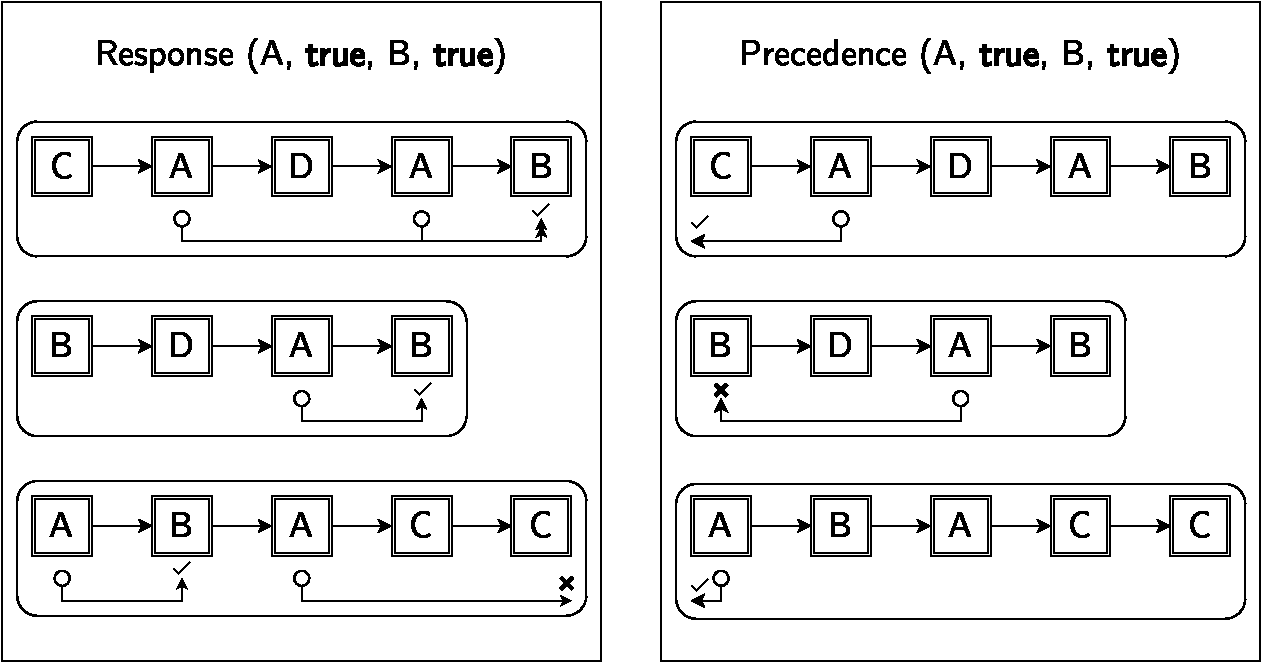
\includegraphics[width=\linewidth]{images/ActivationTargetExample.pdf}
	%	\begin{subfigure}{.27\columnwidth}
		%		\resizebox{\textwidth}{!}{\begin{tabular}{c c} 
				%				\hline
				%				Label & Event \\ 
				%				\hline
				%				\it{a\_a} & audit\_analysis \\
				%				\it{e\_p} & equipment\_purchase \\
				%				\it{p\_r} & patient\_registered \\
				%				\it{p\_d} & patient\_dismissed \\
				%				\hline 
				%		\end{tabular}}
		%	\end{subfigure}
	%\caption{Two exemplifying clauses distinguishing \textsf{Response} and \textsf{Precedence} behaviours. Traces are represented as temporally ordered events associated to activity labels (boxed). Activation  (or target) conditions are here circled (or ticked/crossed). Ticks (or crosses) indicate a (un)successful match of a target condition. For all activations there must be an un-failing target condition; for precedence, we shall consider at most one activation (\S\ref{sec:DAD}). These conditions require the usage of multiple join tests per trace.}
	\caption{Traces describing the events generated by each hospital unit: those are temporally ordered events associated to \textit{activity labels} (boxed). Activated  (or targeted) events here circled (or ticked/crossed). Ticks (or crosses) indicate a (un)successful match of a target condition.}
	\label{fig:comparison}
\end{figure}
Despite this formulation has been already extended so to support correlation constraints \cite{BurattinMS16}, such a solution is affected by the following two deficiencies: first, correlation conditions have to be represented alongside the target condition levels, thus hampering the exploitation of efficient relational database algorithms for correlation conditions via joins. Furthermore, these operators can only assess the validity of one trace at a time while, on the other hand, we might need to assess the satisfiability of multiple traces at the same time by composing partial results returned by every single operator. These operators cannot be directly exploited as query operators, where multiple traces are considered contemporarily. %similarly to the relational algebra operators for relational databases. 
For this reasons, \S\ref{sec:xltlf} proposes a reformulation of such operators. 

%\subsection{Data-Aware Temporal Logic}

\paragraph*{Data-Aware Conformance Checking}
\texttt{Declare Analyzer}\footnote{\url{http://www.promtools.org/doku.php?id=prom611}} \cite{BurattinMS16} proposes one of the latest solutions for conformance checking over data-aware logs. Declare templates are decomposed into \LTLf expressions (as per the last column of Table \ref{tab:dt}), that not only contain event information, but a payload associated to each event per clause. 
%This approach is claimed to be  more optimised than prior works \cite{VanDerAalst2005}.  
Such solution
%While this solution exhibits good performance, it 
does not exploit RDBMS's 
%the 
benefits %that a relational database can provide, 
where %techniques such as 
query optimisations enhance query running times. 
So, no possible performance gains by shared sub-queries 
is considered so to minimize the data access, e.g., by conveniently 
structuring queries in a query plan \cite{BellatrecheKB21}. 
In addition, the authors
scan all of the traces completely for each Declare clause, while our proposed solution minimizes the data access by only accessing the data relevant for running the model-checking query. 
As their solution does not exploit multiple queries running processes, sub-queries or entire clauses appearing multiple times in the model might be recomputed multiple times, thus tampering with the overall running time.
As per their implementation of the \LTLf operators, authors do not exploit efficient relational algebra operators when possible, as full-outer-theta-joins (or theta-joins) for unions (or conjunctions) with correlation conditions.
%
Last, each clause is completely hardcoded and, as they do not support novel templates via the definition of novel \LTLf formulae, as we instead do. The addition of further Declare clauses would require an entirely new implementation. KnoBAB, on the other hand, supports the definition of potential new Declare templates via configuration files loaded at warm-up, %We propose a more generalised solution, where each clause is composed of a combination of unique operators, allowing for any new clause to be included on the fly.
thus enabling a more general result that goes beyond the Declare language and that can be applied to any temporal specification exploiting \LTLf.

A more recent approach \cite{abs-2112-04623} defined specific data structures for a limited support of declarative queries in sublinear-time. Still, this approach has the major shortcoming of pre-computing the possible \textsf{Precedence} or \textsf{Response} queries at loading time. This approach does not scale up for other possible declarative templates, as this might require to extend the data representation  with additional data structures. On the other hand, our proposed approach is query independent and supports all of the possible queries that might be expressed in \xLTLf. Furthermore, this approach supports logs with neither trace nor event payload, thus preventing from easily extending it with activation, target, and correlation conditions involving data predicates. As this approach had a limited query expressive power, it was not considered in our benchmarks.

\paragraph*{Process Mining through Conformance Checking}
Some approaches utilise conformance checking as a mechanism to mine declarative {models}  from an event log: a scoring function tests % by testing 
the validity of each possible clause over each possible trace. %via a scoring function. 
SQLMiner \cite{SchonigRCJM16} {does so via} SQL queries \cite{Schonig15} {where e}ach specified declarative {template} % e.g. \emph{Response}, 
{is} converted into a SQL query. E.g., given the SQL formulation for the \textsf{Response} template, the query returns a table \textsf{(Activation,Target,Score)} where each row $\braket{\textsf{a},\textsf{b},s}$ represents a candidate clause $\Sdeclare{Response}{a}{b}$, and $s$ is its score.
%{Then, the outcome of such a query is a declare clause distinct by different activation and target combination.} 

Each event log, as well as each activation and target activity label for generating the candidate Declare constraints to be tested, are stored in distinct relational tables. While the former are represented in  \textsf{Log(Id,Trace,ActivityId,Event)}, the latter are stored in \textsf{Actions(ActivationId,TargetId)}. The authors consider 
%To achieve this, the event log is {first} loaded into the database as table. {Then, f}or every activation and target combination {of the declarative template, the authors store the candidate activation and target conditions to be tested in another relational table}. {For scoring the validity of each candidate clause}, the authors also calculate 
\textsc{Support} and \textsc{Confidence} scoring functions to determine the precision and reliability of the calculation. Records which do not pass pre-determined \textsc{Support} and \textsc{Confidence} thresholds are filtered out from the data. While SQL also supports data constraints, this solution considers Declare clauses with neither activation, nor target, %, nor correlation conditions}.
%with payload conditions, as well as 
nor correlation ones with payload predicates. This problem is also shared with  more recent approaches where, despite SQL syntax is extended, no evidence of data predicates is given \cite{Polyvyanyy2022}. 

{Despite the authors} exploit %providing additional 
{data} perspectives in `Resource Assignment Constraints' clauses, distinct from the Declare ones, %these additions were only considered  {as 
	only trace payload conditions are considered. Instead, KnoBAB supports payload information and predicate testing {both \emph{per trace}} and \emph{per event} {(see \S\ref{sec:XES})}, which could also be stored in a separate table as SQLMiner suggests, thus providing greater expressiveness per clause.
%
SQLMiner queries can be chained together using \texttt{\textbf{SET UNION}}, though this provides no possibility for testing which are the clauses that are satisfied by the majority of the traces (Max-SAT). These query plans are not optimized as in \cite{BellatrecheKB21}, thus failing at both minimizing the data access
and running multiple shared sub-queries only once.
This is inferior to KnoBAB, which has the ability to process multiple 
declarative clauses from disparate templates. % in the same query plan.
%queries simultaneously. This allows for further optimisation of the query plan, which can exploit common sub-expression \emph{across queries}. This query plan can then be parallelized and processed with batch computation per query layer.

\section{Logical Model}

\subsection{(Intermediate) Result Representation}
Within the computation pipeline, (intermediate) results are represented as a set of triplets $\braket{i,j,L}$ representing that, starting from event $\sigma^i_j$ in trace $\sigma^i$, we might observe activation, target, or correlation conditions in $L$, an ordered vector.  While for activation and target 
we 
preserve 
the matched event id,
correlations keep track of
both the activation and the target condition leading to the satisfaction of a given $\Theta$ predicate (see the next section). This is a sensible representation, as per declarative constraints, it may exist only one possible $\Theta$ predicate. Such triplets are sorted by trace id and event id, and operators manipulating those (\S\ref{sec:xltlf}) guarantee that only one triplet should appear per unique trace and event id. This guarantees efficient join operations across different intermediate results, as well as efficient counting of the satisfied conditions for each trace. %While the former might be implemented via sorted joins, the latter can be achieved by either binary search operations or by look-ahead jumps, as the events pertaining to a trace are contiguous. 
E.g., Clause \Circled{\small C} from \figurename~\ref{fig:knobab_pipeline} requires access to just \textsf{AttributeTable}s, as all of the activity labels are associated to data conditions. {The offset from the attribute tables can then be used to identify the trace and event associated to the data condition (if fulfilled).} When we want to return events for which $\mathcal{P}_{12}$ holds, we need to only consider the data associated to \texttt{Lumpectomy} events having a positive biopsy and levels of CA15.3 greater than 50. This will require the intersection of the events related to biopsy with the ones related to CA15.3. The selected rows are then  converted into the intermediate result representation ad intersected; in this situation, we only obtain $\Set{\braket{3,\mbox{}\mbox{{3}},\{A(\mbox{}\mbox{{3}})\}}}$, as the only event meeting such requirements is the {third} from the third trace. 
As we are going to see in the next paragraph, A is the container of matched activation conditions. 
Similarly, $\mathcal{P}_{8}$ will return $\Set{\braket{\mbox{}\mbox{{1}},\mbox{}\mbox{{3}},\{A(\mbox{}\mbox{{3}})\}}}$, thus obtaining $\Set{\braket{1,\mbox{}\mbox{{3}},\{A(\mbox{}\mbox{{3}})\},\braket{3,\mbox{}\mbox{{3}},\{A(\mbox{}\mbox{{3}})\}}}}$ as a final result associated to \Circled{\small C}: this remarks that only traces \ding{192} and \ding{194} describe patients that underwent a surgical operation under such conditions.

Our proposed representation is different from the one provided by \cite{BurattinMS16} which cannot represent for each event within a trace all the possible activation, target, or join condition happening in the future, as it is impossible to represent single trace events that are not necessarily represented by activation or target conditions. As observed in \S\ref{sec:DAD}, this information is required for checking the satisfiability of $\varphi$ while jointly visiting both the trace (now represented as subsequent rows in the result representation) and the formula. 
In fact, authors exploit
a hash map of hash maps, associating  each trace to the collected activation conditions which, in turn, might be associated with further target conditions. 
This solution is even less efficient than exploiting sorted linear data structures.


\begin{algorithm}
	\caption{\xLTLf pseudocode implementation for the basic timed operators}\label{algo:xltlfAlgo}
	
	
	\begingroup % trick algorithm2e into thinking we're in one column mode
	\csname @twocolumnfalse\endcsname
	\noindent
	\resizebox{\textwidth}{!}{%
		\begin{minipage}{1.4\textwidth}
			%%%%%%%%%%%%%%
			\begin{algorithmic}[1]
				\Statex
				\Function{Future}{$\phi$}
				%\State {\textbf{Require:\;}sorted($\phi$)}
				\ForAll{$\braket{t,e,L}\in\phi$}
				\textbf{yield} $\braket{t,e,\bigcup\Set{L'|\braket{t,e',L'}\in\phi\texttt{\textbf{\;and\;}}e'\geq e}}$
				\EndFor
				\EndFunction\medskip
				%%
				\Function{Globally}{$\phi$}
				%\State {\textbf{Require:\;}sorted($\phi$)}
				\ForAll{$\braket{t,e,L}\in\phi$}
				\State $E\gets\Set{e'|\braket{t,e',L'}\in\phi\texttt{\textbf{\;and\;}}e'\geq e}$
				\IIf {$|E|=\ell_t-e$} 
				\textbf{yield} $\braket{t,e,\bigcup\Set{L'|\braket{t,e',L'}\in\phi\texttt{\textbf{\;and\;}}e'\in E}}$
				\EndIIf
				\EndFor
				\EndFunction\medskip
				%%
				\Function{Next}{$\phi$}
				%\State {\textbf{Require:\;}sorted($\phi$)}
				\ForAll{$\braket{t,e,L}\in\phi$\textbf{\;s.t.} $e>1$}
				\textbf{yield} $\braket{t,e-1,L}$
				\EndFor
				\EndFunction\medskip
				%%
				\Function{CommonJoin}{$\phi,\phi',\Theta,{isDisjunctive}$} %\Comment{Sort Merge (Full-Outer-)Join}
				%\State %{\textbf{Require:\;}sorted($\phi$)\textbf{\;and\;}sorted($\phi'$)}
				\State  $it\gets$\textbf{Iterator}$(\phi), it{'}\gets$\textbf{Iterator}$(\phi')$
				\While{$it\neq\emptyset$\textbf{\;and\;}$it'\neq\emptyset$}
				\State $\braket{t,e,L}\gets\texttt{current}(it)$, $\braket{t',e',L'}\gets\texttt{current}(it')$
				
				
				
				\If{$t=t'$ \textbf{and} $e=e'$}
				\State $L''\gets\emptyset$
				
				\If{$\Theta\neq\textbf{true}$\;\textbf{and}\;$L\neq\emptyset$\;\textbf{and}\;$L'\neq\emptyset$}
				\ForAll{$A(m)\in L$\textbf{\;and\;}$T(n)\in L'$\textbf{\;s.t.\;}$\Theta(m,n)$}
				\State $L''\gets L''\cup\Set{M(m,n)}$
				\EndFor
				\Else
				\State \textbf{if}\;$L=\emptyset$\;\textbf{then}\;$L''\gets\{A(e)\}$\;\textbf{else}\;$L''\gets L$ \State \textbf{if}\;$L'=\emptyset$\;\textbf{then}\;$L''\gets L\cup\{T(e')\}$\;\textbf{else}\;$L''\gets L''\cup L'$
				\EndIf
				
				\State \textbf{if}\;$L''\neq\emptyset$\;\textbf{then\;yield} $\braket{t,e,L''}$; 
				\State $\texttt{next}(it)$; $\texttt{next}(it')$; 
				\ElsIf{$t<t'$\textbf{\;or\;}($t=t'$\textbf{\;and\;}$e<e'$)} 
				\IIf  {$isDisjunctive$} \textbf{yield} $\braket{t,e,L}$  \EndIIf
				\State $\texttt{next}(it)$
				\Else 
				\IIf  {$isDisjunctive$} \textbf{yield} $\braket{t',e',L'}$  \EndIIf
				\State $\texttt{next}(it')$
				\EndIf
				\EndWhile
				\EndFunction\medskip
				%%
				\Function{And}{$\phi,\phi',\Theta$}
				\Call{CommonJoin}{$\phi,\phi',\Theta,\textbf{false}$}
				\EndFunction\medskip
				%%
				\Function{Or}{$\phi,\phi',\Theta$}
				\Call{CommonJoin}{$\phi,\phi',\Theta,\textbf{true}$}
				\EndFunction\medskip
				%%
				\Function{Until}{$\phi,\phi',\Theta$}
				%\State %{\textbf{Require:\;}sorted($\phi$)\textbf{\;and\;}sorted($\phi'$)}
				\ForAll{$t$ \textbf{\;s.t.\;} $\braket{t,i',L'}\in \phi'$}
				\State $\alpha\gets 1$; $Map\gets\{\}$; $i\gets \min_{\iota}\braket{t,\iota,L}\in \phi'$; $I\gets \max_{\iota}\braket{t,\iota,L_I}+1$
				\While{$i< I$}
				\If{$\alpha=i$} \State $\textit{Map}[\alpha]\gets\textit{Map}[\alpha]\cup L'$
				
				\State $i\gets \min_{\iota,\iota>i}\braket{t,\iota,L}$
				\ElsIf{\textbf{exists} $\braket{t,j,L_j}\in \phi$ \textbf{s.t.}\; $j<i$}
				\If{$\braket{t,\alpha,L_\alpha},\braket{t,\alpha+1,L_{\alpha+1}},\dots,\braket{t,i-1,L_{i-1}}\in\phi,$\\\textbf{\;and\;}$\Theta(i,j)$\textbf{\;for all\;}$T(j)\in L_\alpha\cup\dots\cup L_{i-1}$}
				\State $Map[\alpha]\gets Map[\alpha]\cup \Set{M(k,i)|T(k)\in L_\alpha\cup\dots\cup L_{i-1}}$
				\State $i\gets \min_{\iota,\iota>i}\braket{t,\iota,L}\in\phi'$
				\Else \;$\alpha\gets \alpha+1$
				\EndIf
				\Else \;$\alpha\gets i$
				\EndIf
				\EndWhile
				\ForAll{$\braket{i,L}\in \textit{Map}$}
				\textbf{yield} $\braket{t,i,L}$
				\EndFor
				\EndFor
				\EndFunction
			\end{algorithmic}
			%%%%%%%%
		\end{minipage}%
	}% <------------- end of \resizebox
	\endgroup
\end{algorithm}
\subsection{eXTended \LTLf operators}\label{sec:xltlf}
\[\begin{split}
	\phi:=&\;\;\;\textsf{Init}_{A/T}(A,p)\gsep\textsf{End}_{A/T}(A,p)\gsep\textsf{Exists}_{A/T}(n,A,p)\gsep\textsf{Absence}_{A/T}(n,A,p)\\
	&\gsep \textsf{Next}(\phi)\gsep \textsf{Globally}(\phi)\gsep \textsf{Future}(\phi)\gsep \textsf{Not}(\phi)\\
	&\gsep \textsf{Or}(\phi,\phi',\Theta)\gsep \textsf{And}(\phi,\phi',\Theta)\gsep \textsf{Until}(\phi,\phi',\Theta)\\
	&\gsep \textsf{AndGlobally}(\phi,\phi',\Theta)\gsep \textsf{AndFuture}(\phi,\phi',\Theta)\gsep \textsf{AndNextGlobally}(\phi,\phi',\Theta)\\
\end{split}\]
We  extended \LTLf operators (\xLTLf) directly exploited by our pipeline.
Operators in the first line filter traces' events and represent these into the previously-described result representation. 
\textsf{Init} (\textsf{End}) returns the events at the beginning (end) of each trace satisfying the condition $A\wedge p$. Similarly to \cite{BurattinMS16}, each of these operators might be expressed as either an untimed or as a timed specification. Any operator will be considered timed by default when appearing inside a timed operator, like \textsf{Next}, \textsf{Globally}, \textsf{Future}, \textsf{Until}, and any other composed operator from the last line. E.g., In \figurename~\ref{fig:knobab_pipeline}, \textsf{Exists}$(1,\mathcal{P}_3)$ is a shorthand for \textsf{Exists}$(1,\textrm{FollowUp},-\infty<\textup{CA-15.3}<23.5)$, as each atom always associates an activity label to a payload condition. The operator associated to \textsf{Absence}$(1,\mathcal{P}_3)$ is untimed, while the \textsf{Exists}$(1,\mathcal{P}_3)$ descendant of \textsf{Globally} is timed.  While the timed definition returns a tuple $\braket{i,j,L}$ for each possible event $\sigma^i_j$ within the trace $\sigma^i$ where the formula holds, the untimed specification only checks whether the formula holds at the beginning of the trace. E.g., untimed \textsf{Exists} (\textsf{Absence}) returns the first event trace if at least $n$ (at most $n-1$) events satisfy $A\wedge p$, while the timed version returns the events satisfying (not satisfying) $A\wedge p$ (always $n=1$). All of these operators might be optionally marked as returning either an activation ($A$) or a target ($T$) condition, so that each  $\braket{i,j,L}$ triplet has $L=\{A(j)\}$ or $L=\{T(j)\}$; when no mark is specified, $L$ is empty. To wrap up the previous example, the timed  \textsf{Exists}$(1,\mathcal{P}_3)$ will list the events where $\mathcal{P}_3$ happened, $\Set{\braket{1,3,\{A(3)\}}}$, while the untimed version will just list the traces where such event happened and collect the event of interests in $L$. %, $\Set{\braket{1,1,\{3\}}}$.


The next two lines report the same operators described in \S\ref{sec:DAD} with the addition of the explicit correlation conditions over activation and target conditions for each binary operator. Algorithm~\ref{algo:xltlfAlgo} provides  implementations of the timed versions of such operators, due to lack of space untimed versions are not provided, yet available in our codebase: please observe that $\textsf{Next}(\phi)$ keeps unaltered the activation and target conditions from $\phi$ and just returns the events where $\phi$ happens as a subsequent step. Any binary operator supports $\Theta$ conditions:  \textsf{And} (and \textsf{Or}) can be expressed as a (full-outer-)$\Theta$-join algorithm over the activation and target conditions stored in $L$ associated with the same event. If at least one activation condition matches one target condition from the same event, those are expressed as a marked correlation condition $M(i,j)$ which is then returned by the join. Regarding the same \textsf{Choice} clause from \figurename~\ref{fig:knobab_pipeline}, the correlation condition $\Theta$ associated to \textsf{Or} is then computed for each activation/target match, and if the condition is passed, the resulting match is added to $L$. 


The remaining operators merge multiple operators together when 
a specific implementation outperforms
the execution of the operators separately:
 e.g., $\textsf{AndFuture}(\phi,\phi',\Theta)$ is equivalent to\\ $\textsf{And}(\phi,\textsf{Future}(\phi'),\Theta)$, but preliminary experiments reveal that the former has a more efficient implementation than computing the latter. This choice was inspired by relational algebra, where $\theta$-joins are usually more efficient than performing a join and a selection operation separately.
 On the other hand, % Similarly,  we can associate the correlation condition to implication operators after rewriting 
 $\textsf{Implies}(\phi,\phi',\Theta)$ is rewritten as $\textsf{Or}(\textsf{Not}(\phi),\,\textsf
{And}(\phi,\phi',\Theta),\,\textbf{true})$. As per previous discussion, the left leaf of \textsf{AndFuture}$_\Theta$ in \figurename~\ref{fig:knobab_pipeline} returns all of the referral events with CA 15-3 above the safeguard levels, $\Set{\braket{1,\mbox{}\mbox{{2}},\{A(\mbox{}\mbox{{2}})\}},\braket{3,\mbox{}\mbox{{2}},\{A(\mbox{}\mbox{{2}})\}}}$, while the right leaf returns just the follow-up events below such levels, $\Set{\braket{1,\mbox{}\mbox{{4}},\{A(\mbox{}\mbox{{4}})\}}}$. The operator \textsf{AndFuture}$_\Theta$ will then return only $\Set{\braket{\mbox{}\mbox{{1}},\mbox{}\mbox{{2}},\{M(\mbox{}\mbox{{2}},\mbox{}\mbox{{4}})\}}}$, as only the first trace will have a decrease below the safeguard levels from referral to follow-up.
%
Each \xLTLf operator is going to both return and/or accept data in the result representation, thus making such operators closed on such format.






\section{KnoBAB Architecture}\label{sec:karch}
The methodology behind its design systematically follows the major architectural components of a relational database, with the only bespoke characteristics of tailoring such solution to the specific problem that we intend to solve (\S\ref{ssec:xltlf}), that is, computing either the Max-SAT for each log trace,  or the \textsc{Confidence}/\textsc{Support} associated to each model clause, or computing the traces satisfying all of the model clauses (\textit{conjunctive query}).


\subsection{Data Loading}\label{ssec:dl}
The data loading phase   loads logs  serialized in multiple  formats, thus including the XML-based XES standard, a tab-separated events' activity labels, and the \textsc{Human Readable Log Format} (HRLF) firstly introduced in \cite{bpm21}. We use different data parsers, which are still linked to the same data loading primitives.   
{HRLF also supports the \textsf{bool} data type. This is represented as an integer, where: $val < 1.0 = false,  val \ge 1.0 = true$. In \figurename~\ref{fig:knobab_pipeline}, \textsf{booleans} are displayed in their traditional way (both in the payload and for activation/target conditions), though this is for visual purposes only E.g., \textsf{Exists}$(1,\textrm{Referral},biopsy = true)$ in our pipeline is \textsf{Exists}$(1,\textrm{Referral},\textup{biopsy}\ge 1.0)$.}

If the log does not contain data payloads, the entire log can be represented into two relational tables, \textsf{CountingTable(ActivityId,Trace,\\Count)} and \textsf{ActivityTable(ActivityId,Trace,Event,Prev,Next)}. While the former counts the occurrence of each activity label in $\Sigma$ for each trace, the latter lists all of the possible events similarly to SQLMiner. Both tables compactly represent the initial three columns as a 64-bit unsigned integer, which is also used to sort the tables in ascending order. A row $\braket{\textsf{a},j,h}$ from \textsf{CountingTable} states that there are $h$ events exhibiting the activity label $\textsf{a}$ in the trace $\sigma^j$; each row $\braket{\textsf{a},j,i,q,q'}$ from \textsf{ActivityTable} states that the $i$-th event of the $j$-th trace ($\sigma^j_i=\braket{\textsf{a},p}$) is labelled as $\textsf{a}$, while $q$ (or $q'$) is the pointer to the immediately preceding $\sigma^j_{i-1}$ (or  following, $\sigma^j_{i+1}$) event within the trace if any. \texttt{NULL}s from  \figurename~\ref{fig:knobab_pipeline} in \textsf{ActivityTable} highlight the start (finish) event of each trace, where there is no possible reference to past (future) events. Trace payload information is injected (as an event) before the first event, which is also contained:  all trace payload events contain \texttt{NULL} as \textsf{Prev}. %in all of their previous fields.


If, on the other hand, the log is associated to either trace or event payloads, we exploit 
the query and memory-efficient  column-based model \cite{IdreosGNMMK12}, thus representing all of the values $v$ associated to a  payload key $k$ within the rows from  \textsf{AttributeTable$k$}. In our implementation, each row $\braket{\textsf{a},v,i}$ from  \textsf{AttributeTable$k$(ActivityId,Value,Offset)} represents a value $v$ associated to the key $k$, where $i$ determines the location where the event containing the accessed value is located in \textsf{ActivityTable}; this % where this event occurred, 
provides the trace id and event id required for the intermediate representation.
 To perform payload-based queries efficiently, the table is sorted in ascending order by the  three columns. As each data condition is always associated with a given activity label, those can be effectively run as data range queries run via binary search algorithms. From \figurename~\ref{fig:knobab_pipeline}, all the attributes are stored in distinct tables. \textsf{{Value}} can contain multiple data types, but each attribute is associated to only one type. %When decomposed atoms are used for a query, the tables associated with the query are then accessed. %The offset value can then determine : 


\textsf{CountingTable} is mainly accessed for existential and \textsf{Exists} and \textsf{Absence} templates where no data payload is specified, while  \textsf{ActivityTable} is  used for either returning all of the events within the log associated to a given activity label or returning all of the events happening at either the beginning or at the end of a trace. Each table \textsf{AttributeTable$k$}, on the other hand, will 
return all the events satisfying a given condition associated with a specific %data 
key $k$. 

After loading the whole dataset, the number of the traces within the log $|\mathcal{L}|$, the length $\ell_j$ for each trace $\sigma^j$, and the number of distinct activity labels $|\Sigma|$ is known. Given this, we can get the number of occurrences of each $i$-th activity label from $\Sigma$ in each trace by directly accessing the rows within the \textsf{CountingTable} in \figurename~\ref{fig:knobab_pipeline} are within the range $[|\mathcal{L}|\cdot (i-1) + 1,\; |\mathcal{L}|\cdot i]$. The offsets for accessing the \textit{Mastectomy} activity label in \textsf{CountingTable} is $[3 \cdot (4-1) + 1, 3 \cdot 4] = [10,12]$. Given that this counting table computes only for untimed operations, the intermediate result for untimed \textsf{Exists}$_A(1,\textit{Mastectomy},\textbf{true})$ is $\Set{\braket{1,1,\emptyset}}$, as only \ding{192} contains such an event.
%
On the other hand, the loading and indexing phase generates an \textsf{ActivityTable} associated with two indices, a primary and a secondary index. While the former returns all of the events associated with a specific activity label, the latter accesses either the first or the last event in a trace. Pointers associated with each record enable  traces' temporal scan. 
%Loading and indexing algorithms are omitted due to the page limits.
%<<<<<<< HEAD
%>>>>>>> 3a6e4d5b1f0a9d9f27e0e9f9588e3f0f743bda2c
%=======
%>>>>>>> main
%>>>>>>> b69bdd98c4f898e5f4801fc44cbae460ecd04aef




\subsection{Query Compiler}\label{sec:qc}
The query compiler is structured into three main phases. \textit{(i)} The \textit{atomization pipeline}  rewrites the data predicates 
associated with each activity label as a 
disjunction of mutually exclusive data conditions. We can tune KnoBAB to always atomize each possible activity label if it exists any Declare Constraint associating it to a data condition as in \cite{bpm21}, or we can choose to provide such an interval decomposition only to the Declare constraints exhibiting data conditions. While the former approach will maximise the access to the \textsf{AttributeTable}s, the latter will maximise the access to the \textsf{ActTable}. By doing so, we can ensure that the data satisfying some given properties can be visited at most once, thus guaranteeing the assumptions from \cite{BellatrecheKB21} also at the data accessing level. Correlation conditions do not undergo this rewriting step. The atomized model in \figurename~\ref{fig:knobab_pipeline} replaces the non-correlation data predicates with the outcome of the atomization process as in \cite{bpm21}. 


We \textit{(ii)} rewrite each Declare constraint as a \xLTLf formula, where the activations (and the potential target) conditions are instantiated with either just activity labels or also with associated data conditions as per the previous atomization step. 
Each sub-expression appears at most once as in \cite{BellatrecheKB21} by representing every single node in the query plan at most once: this is ensured by an internal query manager cache. The resulting query plan considering the simultaneous execution of multiple queries can be represented as a \textsc{Direct Acyclic Graph} (DAG).  
For each declarative clause appearing more than once (e.g., $m>1$), the associated \xLTLf expression will be computed at most  once, while its resulting data is going to be accessed $m$ times by the final aggregator: as per \figurename~\ref{fig:knobab_pipeline}, despite \textsc{Response} might be considered a subquery of \textsc{Succession}, the Max-SAT is still going to retrieve the output provided by the associated sub-expression. Green arrows remark operators' output shared among operators. Please also observe that operators with the same name and arguments but marked either with activation, target, or no specification are considered different as they provide different results, and therefore are not merged together. 
%\textit{Second}, we rewrite each Declare constraint as a \xLTLf formula, where the activations (and the potential target) conditions are instantiated with either just activity labels or also with associated data conditions as per previous atomization step. This step is mediated through a configuration file loaded at warm-up time, where novel declare constraints can be expressed as \xLTLf formulae. We guarantee to represent each subquery at most once as in \cite{BellatrecheKB21} by representing each node in the query plan at most once: this is ensured by an internal cache. At the end of this process, the query plan considering the simultaneous execution of multiple queries can be represented as a \textsc{Direct Acyclic Graph} (DAG). 
%>>>>>>> main
%>>>>>>> b69bdd98c4f898e5f4801fc44cbae460ecd04aef
This includes distinctions between timed and untimed operators.

Given that our execution engine provides the possibility of running a query plan in either a parallel or a sequential mode, we need   an additional step. \textit{(iii)} The previous DAG  represents a dependency graph, where a link between an ancestor and one of its descendants implies that the latter has to be computed before the former, thus suggesting an execution order. \figurename~\ref{fig:knobab_pipeline} depicts this as an arrow starting from the ancestor. To enforce that, we perform a lexicographical order over the DAG, through which we compute the maximum depth level associated with each node of the graph. %After doing so, 
We then represent the query graph as a stack of depth levels, where each operator on it can be run in parallel alongside its siblings.
 This proves that the computation of Declare Clauses can be reduced into an embarrassingly parallel problem, as the layered execution guarantees that no thread communication needs to happen, and that multiple threads could access contemporary the partial results associated with the immediately-descendant operators, as the former will return all of the events where the condition happened, while the latter will just return the trace event satisfying such condition alongside the required activations/targets listed in $L$. Furthermore, the proposed parallelization ensures minimizing the data access for computing the query. The DAG \figurename~\ref{fig:knobab_pipeline} depicts a query plan.

%\subsection{In-Memory Storage Manager}

\subsection{Execution Engine} \label{ssec:xltlf}
At the time of the writing, KnoBAB supports four different types of model aggregation queries: Conjunctive Query, Max-SAT, \textsc{Confidence}, and \textsc{Support}. As we will see at the end of the subsection, these will not require a change on the query plan, but just a different way to integrate the intermediate representation $\phi_i$ returned by each declarative clause $c_i$. 


\textit{First}, the execution engine takes both the relational database resulting from the data loading and the DAG returned by the query compiler, and uses the leaf nodes from the latter to access the former. By query plan construction, all of the relevant data parts are going to be accessed at most once and then transformed into the expected intermediate result representation. \textit{Second}, the intermediate results are propagated from the leaves towards each root node associated with a declarative clause $c_k$. Any intermediate representation is always associated with each operator returning it as a temporary primary-memory cache. Each intermediate cache  might be completely freed if we are not computing a  \textsc{Confidence} query and if the furthest ancestor has already accessed it, or if it is a cache non-associated to an activation required by \textsc{Confidence} and the furthest ancestor has already accessed it. \textit{Third}, when the computation will finish running the shallowest DAG depth level containing the \xLTLf root associated with the entry-point of each declarative clause $c_k$, each of these operators will have an intermediate result $\phi_k$ stating all the traces satisfying $c_k$.

The {Conjunctive Query} will return the traces satisfying all of the Declare clauses via the intersection of all of the clauses via \textsf{And} and \textbf{true} as a $\Theta$ condition. Max-SAT will count, for each log trace $\sigma_i$, the intermediate results $\phi_k$ associated with each clause $c_k$ containing it, and then provide the ratio of such value over the total number of the model clause $|\mathcal{M}|$. By denoting as $\textsf{ActLeaves}(\phi_k)$ the untimed union of the intermediate results returned by the activation conditions for the declare clause $c_k\in\mathcal{M}$, the \textsc{Confidence} for $c_k$ is the ratio between the total number of traces returned by $\phi_k$ and the overall traces containing an activation condition. Dividing the total number of traces returned by $\phi_k$ by the total log traces returns the \textsc{Support}. Once each $\phi_k$ per clause $c_k$ is computed, the aggregation functions can be then expressed as follows:
\[\textup{ConjQuery}(\phi_1,\dots,\phi_n)=\textsf{And}(\phi_1,\dots\textsf{And}(\phi_{n-1},\phi_n,\textbf{true}),\textbf{true})\]
\[\textup{Max-SAT}(\phi_1,\dots,\phi_n)=\left(\frac{|\Set{k|\exists j,L. \braket{i,j,L}\in\phi_k}|}{|\mathcal{M}|}\right)_{\sigma^i\in \mathcal{L}}\]
\[\textsc{Confidence}(\phi_1,\dots,\phi_n)=\left(\frac{|\Set{i|\exists j,L. \braket{i,j,L}\in \phi_k}|}{|\textsf{ActLeaves}(\phi_k)|}\right)_{c_k\in \mathcal{M}}\]
\[\textsc{Support}(\phi_1,\dots,\phi_n)=\left(\frac{|\Set{i|\exists j,L. \braket{i,j,L}\in \phi_k}|}{|\mathcal{L}|}\right)_{c_k\in \mathcal{M}}\]
As the user in \figurename~\ref{fig:knobab_pipeline} asks the ratio between satisfied clauses over the model size, the query plan exhibits a Max-SAT aggregation.



\begin{algorithm}
	\caption{LTL$_f$ pseudocode implementation for the basic timed operators}


\begingroup % trick algorithm2e into thinking we're in one column mode
\csname @twocolumnfalse\endcsname
\noindent
\resizebox{\textwidth}{!}{%
	\begin{minipage}{1.3\textwidth}
%%%%%%%%%%%%%%
	\begin{algorithmic}[1]
		\Statex
\Function{Future}{$\varphi$}
		\State {\textbf{Require:\;}sorted($\varphi$)}
		\ForAll{$\braket{t,e,L}\in\varphi$}
		 \textbf{yield} $\braket{t,e,\bigcup\Set{L'|\braket{t,e',L'}\in\varphi\texttt{\textbf{\;and\;}}e'\geq e}}$
		\EndFor
\EndFunction\medskip
%%
\Function{Globally}{$\varphi$}
		\State {\textbf{Require:\;}sorted($\varphi$)}
		\ForAll{$\braket{t,e,L}\in\varphi$}
		\State $E\gets\Set{e'|\braket{t,e',L'}\in\varphi\texttt{\textbf{\;and\;}}e'\geq e}$
		\If {$|E|=\ell_t-e$} 
		 \textbf{yield} $\braket{t,e,\bigcup\Set{L'|\braket{t,e',L'}\in\varphi\texttt{\textbf{\;and\;}}e'\in E}}$
		 \EndIf
		\EndFor
\EndFunction\medskip
%%
\Function{Next}{$\varphi$}
		\State {\textbf{Require:\;}sorted($\varphi$)}
		\ForAll{$\braket{t,e,L}\in\varphi$\textbf{\;s.t.} $e>1$}
		\textbf{yield} $\braket{t,e-1,L}$
		\EndFor
\EndFunction\medskip
%%
\Function{CommonJoin}{$\varphi_1,\varphi_2,\Theta,{isDisjunctive}$} %\Comment{Sort Merge (Full-Outer-)Join}
	\State {\textbf{Require:\;}sorted($\varphi_1$)\textbf{\;and\;}sorted($\varphi_2$)}
	\State  $it\gets$\textbf{Iterator}$(\varphi_1), it\gets$\textbf{Iterator}$(\varphi_2)$
	\While{$it\neq\emptyset$\textbf{\;and\;}$it'\neq\emptyset$}
	\State $\braket{t,e,L}\gets\texttt{current}(it)$, $\braket{t',e',L'}\gets\texttt{current}(it')$
	\If{$t=t'$ \textbf{and} $e=e'$}
	\If{$L=\emptyset$} $L''\gets L'$
	\ElsIf{$L'=\emptyset$} $L''\gets L$
	\Else 
	\State $L''\gets\emptyset$
	\ForAll{$m\in L$\textbf{\;and\;}$n\in L'$\textbf{\;s.t.\;}$\Theta(m,n)$}
	\State $L''\gets L''\cup\Set{\textbf{join}[m,n]}$
	\EndFor
	\EndIf
	\State \textbf{yield} $\braket{t,e,L''}$; $\texttt{next}(it)$; $\texttt{next}(it')$; 
	\ElsIf{$t<t'$\textbf{\;or\;}($t=t'$\textbf{\;and\;}$e<e'$)} 
	\If  {$isDisjunctive$} \textbf{yield} $\braket{t,e,L}$  \EndIf
	\State $\texttt{next}(it)$
	\Else 
		\If  {$isDisjunctive$} \textbf{yield} $\braket{t',e',L'}$  \EndIf
		\State $\texttt{next}(it')$
	\EndIf
	\EndWhile
\EndFunction\medskip
%%
\Function{And}{$\varphi_1,\varphi_2,\Theta$}
	\Call{CommonJoin}{$\varphi_1,\varphi_2,\Theta,\textbf{false}$}
\EndFunction\medskip
%%
\Function{Or}{$\varphi_1,\varphi_2,\Theta$}
\Call{CommonJoin}{$\varphi_1,\varphi_2,\Theta,\textbf{true}$}
\EndFunction\medskip
%%
\Function{Until}{$\varphi_1,\varphi_2,\Theta$}
\State {\textbf{Require:\;}sorted($\varphi_1$)\textbf{\;and\;}sorted($\varphi_2$)}
\ForAll{$t$ \textbf{\;s.t.\;} $\braket{t,i',L'}\in \varphi_2$}
\State $\alpha\gets 0$; $Map\gets\{\}$
\ForAll{$\braket{t,i,L}\in\varphi_2$}
\While{$i<\alpha$}
\If{$\braket{t,\alpha,L_\alpha},\braket{t,\alpha+1,L_{\alpha+1}},\dots,\braket{t,i-1,L_{i-1}}\in\varphi_1,$\\\textbf{\;and\;}$\Theta(\alpha,j)$\textbf{\;for all\;}$j\in L_\alpha\cup\dots\cup L_{i-1}$}
\State $Map[i]\gets\Set{\texttt{\textbf{join}[k,i]}|k\in L_\alpha\cup\dots\cup L_{i-1}}$
 
\EndIf
\EndWhile
\State $Map[i]\gets Map[i]\cup L$; 
\ForAll{$i\in \texttt{mapKey}(Map)$} \textbf{yield} $\braket{t,i,Map[i]}$
\EndFor
\EndFor
\EndFor
\EndFunction\medskip
	\end{algorithmic}
%%%%%%%%
\end{minipage}%
}% <------------- end of \resizebox
\endgroup
\end{algorithm}
\subsection{LTLf Operators' implementation on the Physical Model}
\begin{table}[!t]
\resizebox{\linewidth}{!}{
	\begin{tabular}{ l l r r r }
		\toprule
		Competitor & Dataset & Traces $|\mathcal{L}|$ & Events & Distinct Activities $|\Sigma|$\\ [0.5ex] 
		\midrule
		\multirow{4}{*}{SQL Miner} &
		BPIC 2011 (original) & 1143 & 150 291 & 624 \\ &
		BPIC 2011 (10) & 10 & 2613 & 158 \\ &
		BPIC 2011 (100) & 100 & 12 195 & 276 \\ &
		BPIC 2011 (1000) & 1000 & 133 935 & 607 \\ 
		\midrule
		\multirow{1}{*}{Declare Analyzer} &
		BPIC 2012 (original) & 13087 & 262 200 & 24 \\
		\bottomrule
	\end{tabular}
}
\caption{Range of datasets used for benchmarking.}
\label{table:dataset}
%\vspace{-10mm}
\end{table}
\section{Experimental Analysis}\label{sec:exp}
Our benchmarks exploited a Razer Blade Pro on Ubuntu 20.04: Intel Core i7-10875H CPU @ 2.30GHz - 5.10 GHz, 16GB DDR4 2933MHz RAM, 180GB free disk space. Our datasets (\tablename~\ref{table:dataset}) include 2 real life event logs\footnote{\url{https://dx.doi.org/10.17605/OSF.IO/XWD3V}\label{footnote:datasets}}: \textsf{BPIC 2011} (Dutch academic hospital log) and \textsf{BPIC 2012 } (Dutch loan company).




\subsection{SQLMiner}\label{ssec:sqlmin}
These experiments want to test our working hypotheses for the possibility of engineering a tailored relational database architecture that can outperform process mining through conformance checking running on traditional relational databases. In the latter, no \LTLf operators are exploited but a table similar to \texttt{ActivityTable} is exploited. % are provided and non-customary tabular representation is exploited. 
Given that the SQL provided in \cite{Schonig15,SchonigRCJM16} might only return the \textsc{Support} associated with each candidate Declare clause (\texttt{SQLMiner+Support}), we provided the least possible changes to also associate each candidate clause with the set of all the traces satisfying it. This was achieved by both extending the activation condition expressed in SQL and using \texttt{array\_aggr} included in \textbf{PostgreSQL 14.2} to list such traces (\texttt{SQLMiner+TraceInfo}). For comparing the same settings in KnoBAB, we run both Max-SAT and \textsc{Support} queries with the difference that, in our case, both of these implementations will always return, per intermediate result specification, the trace information satisfying each possible model clause.
For our experiments, we exploited {BPIC 2011} dataset from \cite{SchonigRCJM16}. To test the scalability of the solutions, we recorded the query's runtime with increasing log size: we randomly sampled the log with three sub-logs containing 10, 100 and 1000 traces, while guaranteeing that each sub-log is always a subset of the greater ones. For each sub-log, we generated 8 distinct models as benchmarked in \cite{Schonig15}. Each model consists of 25 clauses instantiating the same Declare template (\textit{elected template}) with different activation and target conditions. Those did not consider payload conditions and were only considering the most frequent activity labels appearing in the sub-log. Models of greater size  caused an exponential increase in required secondary memory for SQLMiner (on the order of TB), justifying our approach for a sampled model. In their approach, each model was queried by running the SQL query corresponding to the \textit{elected template}, and the specific activation and target conditions from the model's clauses were distinct rows in the \textsf{Action} table.


\begin{figure}[!t]
	\hspace*{-3mm}
	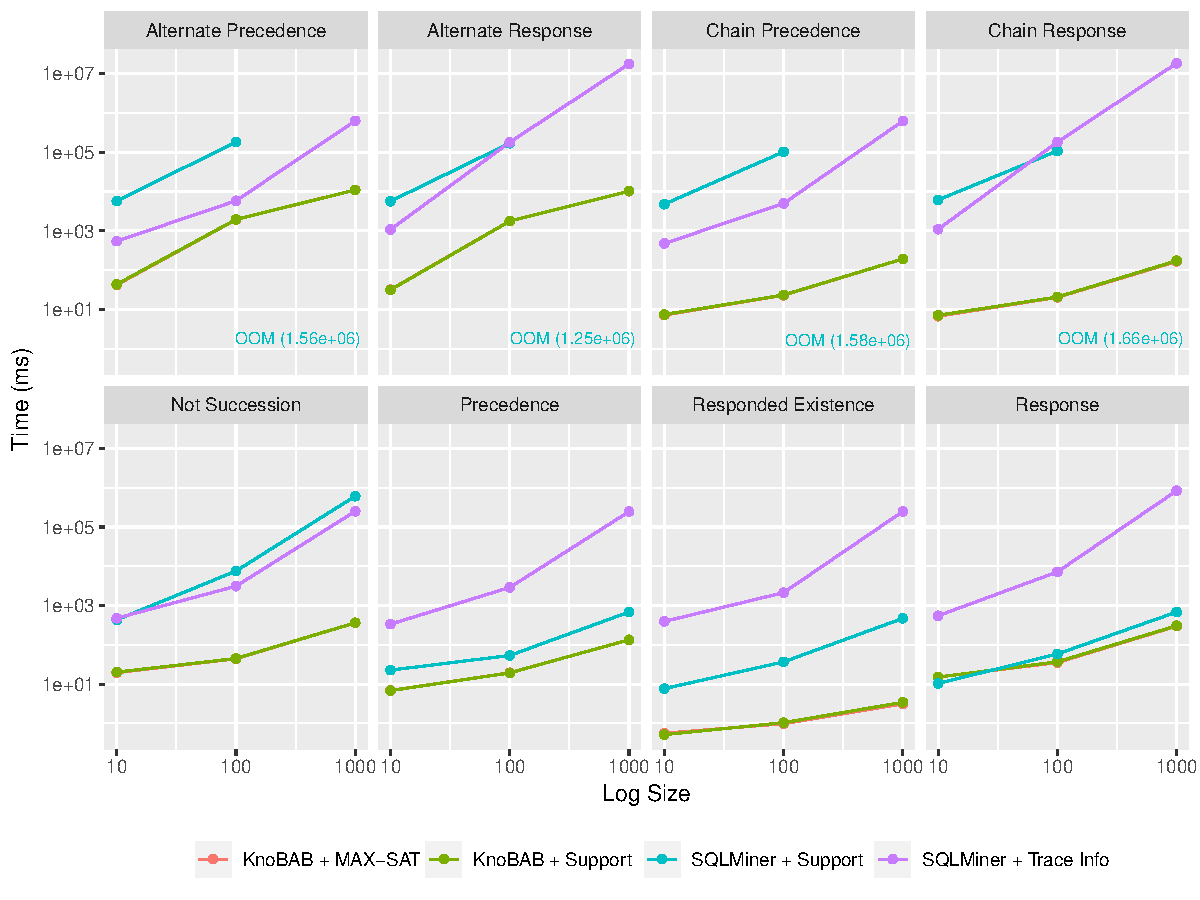
\includegraphics[width=1.05\linewidth]{images/sqlminer_benchmark.pdf}
	\caption{KnoBAB vs SQLMiner Performance for 25 clauses with frequent activity labels with Support and Trace Information. OOM indicates Out of Secondary Memory for logs containing $10^3$ traces (followed by the time taken for an exception to occur).}\label{fig:vsSQL}
	\vspace{-5mm}
\end{figure}
The outcome of such experiments is represented in \figurename~\ref{fig:vsSQL}, where each plot represents the running time associated with models containing the same \textit{elected template}. In the worst-case scenario (\textsf{Response}), we exhibit similar query running times to SQLMiner. Even so, we are always providing trace information, and in the case of \textsf{Response}, altering the SQL to provide this causes over an order of magnitude increase in complexity. In the best-case scenario, we outperform SQLMiner by at most 5 orders of magnitude. This is because our query plan minimizes the access to the data queries and our computation avoided explicit computations of aggregations. This was achieved by sorting the intermediate results, and, as our operators' implementations guarantee that (intermediate) results are always sorted, counting operations are just linear scans of the intermediate result representation. Our solution never exceeded the 16GB of primary memory while, for some more complex queries (top row of \figurename~\ref{fig:vsSQL}), SQLMiner exceeded it, thus proving that our solution is also memory efficient. One of the outstanding examples is \textsf{RespExistence}, where we are greatly more efficient than SQLMiner. This is a clear indicator of the potential gains from utilising our proposed \textsf{CountTable}, summarizing the appearance of activity labels in events per trace by counting their instances. The original SQL query is required to scan the whole \texttt{Log} table (similar to our \texttt{ActivityTable}), which contained all of the trace events. We also remind the reader that the \textsf{CountTable} can be efficiently created while scanning the whole log dataset, so no super-linear overhead is added at loading time. This further validates that an adequate tabular representation twinned with \xLTLf operators extending the \LTLf specification for tabular data provides a suitable solution. Last, the running time of the Max-SAT problem and \textsc{Support} for KnoBAB exhibited similar running times, while in PostgreSQL those exhibit huge variations depending on the query-plan rewriting performed by the PostgreSQL query engine. For some elected templates, our proposed \texttt{SQLMiner+TraceInfo} formulation proved also to be more efficient than the \texttt{SQLMiner+Support} queries originally proposed by \cite{Schonig15} (which contain no trace information).




\begin{figure}[!t]
		\centering
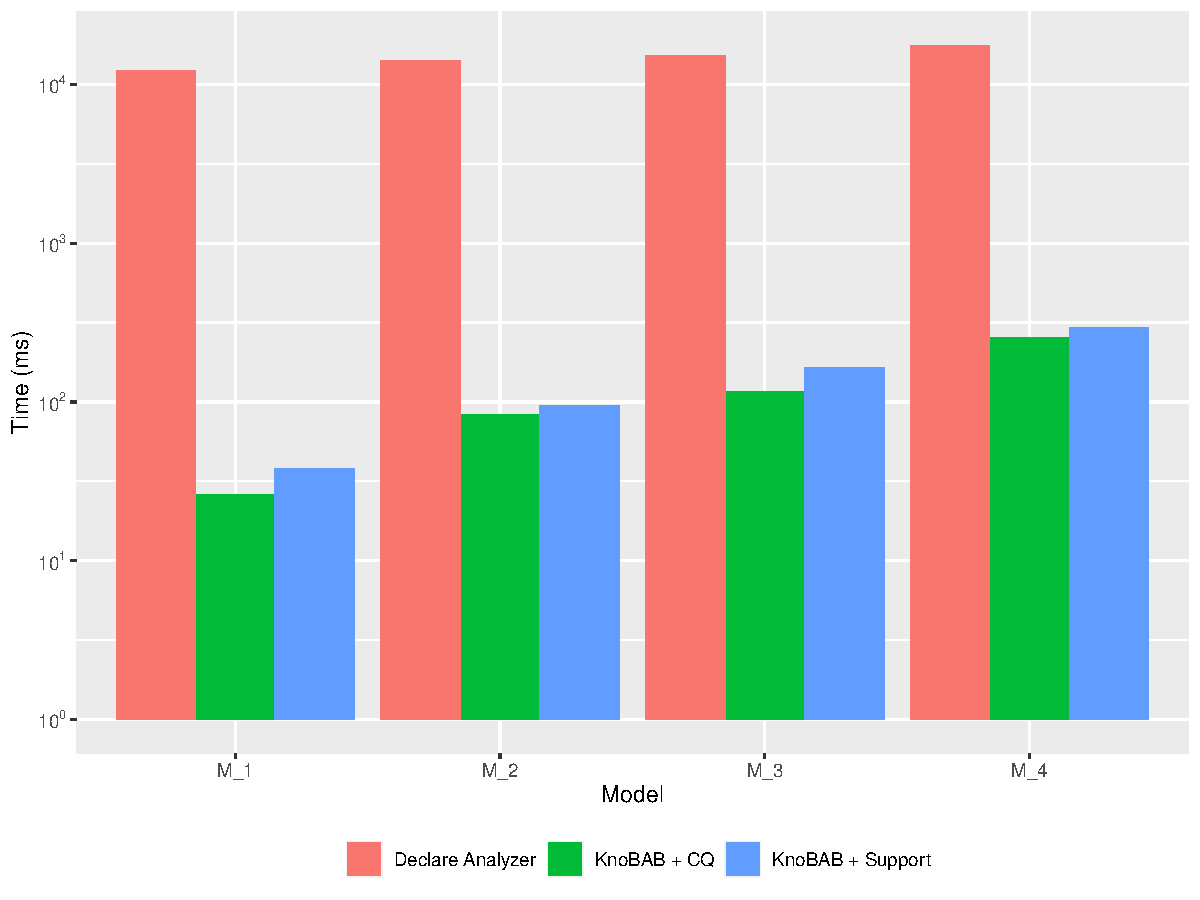
\includegraphics[width=.71\linewidth]{images/burattin_benchmark.pdf}
\captionof{figure}{KnoBAB vs Declare Analyzer Performance. %for Different Models. %Knobab + CQ indicates the intersection, per trace, of all the satisfaction result representations i.e. returning  the traces that fulfilled all the clauses.
}\label{fig:vsBuatto}
\end{figure}

\subsection{Declare Analyzer}\label{ssec:declan}
The set of experiments on Declare Analyzer have the aim of comparing our proposed solution against a solution tailored for solving Declare Conjunctive Queries over logs running exclusively in primary memory. We chose to exploit via MapDB\footnote{\url{https://mapdb.org/}} for log representation, thus making it more similar to a relational database. %In particular, we want to show the benefit of running a query plan when multiple sub-queries are shared: by increasing the size of the model by adding novel queries, we are expecting that while our solution exhibits a near constant running time, Declare Analyzer's running time should increase almost linearly as per the authors' claim.
%=======
%>>>>>>> 33357ef815c5a234b684fdafdceed45bf3a89be0
%In order to do so, 
We exploited the {BPIC 2012} dataset, defined in \tablename~\ref{table:dataset}, also used in \cite{BurattinMS16}. {The data was modified so as to efficiently act across the trace payload information. \cite{BurattinMS16} requires the injecting of trace payload information into \textit{each} event. Our implementation, as stated in \ref{sec:XES}, injects the trace payload as a unique event at the beginning of the trace. } %\remove{and we slightly edited the queries}
 The queries (from the same paper) %\remove{in the same paper} 
 were edited\footnoteref{footnote:datasets}, where all the models $M_i$ and $M_j$ with $i<j$ are always the former a subset of the latter, while $M_{i+1}$ increases by 5 from %\remove{-fold}
   $M_i$. 
%
%\begin{table}[!b]
%	\resizebox{\linewidth}{!}{
%		\begin{tabular}{ll}
%			Model & Queries \\
%			\toprule
%			\multirow{5}{*}{$M_1=\qquad$} \rdelim\{{5}{3mm} & $q_{1}:= \DeclareClause{Response}{A\_SUBMITTED}{\textbf{true}}{A\_ACCEPTED}{\textbf{true}}$ \\ & $q_{2}:= \DeclareClause{Response}{A\_SUBMITTED}{\texttt{AMOUNT\_REQ} \geq 10^3}{A\_ACCEPTED}{\textbf{true}}$ \\&
%			$q_{3}:= \DeclareClause{Response}{A\_SUBMITTED}{\texttt{AMOUNT\_REQ} < 10^3}{A\_ACCEPTED}{\textbf{true}}$ \\&
%			$q_{4}:= q_{1} \textrm{ where } \texttt{A\_SUBMITTED.org:resource}=\texttt{A\_ACCEPTED.org:resource}$ \\&
%			$q_{5}:= q_{1} \textrm{ where } \texttt{A\_SUBMITTED.org:resource}\neq\texttt{A\_ACCEPTED.org:resource}$ \\
%			\toprule
%			\multirow{5}{*}{$M_2=M_1+$}\rdelim\{{5}{3mm} & $q_{6}:= \DeclareClause{Response}{W\_Completeren aanvraag}{\textbf{true}}{W\_Valideren aanvraag}{\textbf{true}}$ \\ &
%			$q_{7}:= \DeclareClause{Response}{W\_Completeren aanvraag}{\textbf{true}}{O\_CANCELLED}{\textbf{true}}$ \\&
%			$q_{8}:= q_{6} \textrm{ where } \texttt{W\_Valideren aanvraag.org:resource}\neq\texttt{W\_Valideren aanvraag.org:resource}$ \\&
%			$q_{9}:= \DeclareClause{Response}{W\_Valideren aanvraag}{\texttt{AMOUNT\_REQ} = 5 \cdot 10^3}{O\_CANCELLED}{\textbf{true}} $ \\&
%			$q_{10}:= q_{9} \textrm{ where } \texttt{W\_Valideren aanvraag.org:resource}=\texttt{O\_CANCELLED.org:resource}$ \\
%			\toprule
%			\multirow{6}{*}{$M_3=M_2+$}\rdelim\{{6}{3mm} & $q_{11}:= \DeclareClause{Response}{O\_SELECTED}{\textbf{true}}{O\_CANCELLED}{\textbf{true}}$ \\&
%			$q_{12}:= q_{11} \textrm{ where } \texttt{O\_SELECTED.org:resource}=\texttt{O\_CANCELLED.org:resource}$ \\&
%			$q_{13}:= \DeclareClause{Response}{O\_SELECTED}{\texttt{AMOUNT\_REQ} < 8 \cdot 10^3}{O\_CANCELLED}{\textbf{true}}$ \\&
%			$q_{14}:= q_{13} \textrm{ where } \texttt{O\_SELECTED.org:resource}=\texttt{O\_CANCELLED.org:resource}$ \\&
%			$q_{15}:= \DeclareClause{Response}{O\_SELECTED}{\texttt{AMOUNT\_REQ} > 10^3}{O\_CANCELLED}{\textbf{true}}$ \\&
%			\qquad\; $\textrm{ where } \texttt{O\_SELECTED.org:resource}\neq\texttt{O\_CANCELLED.org:resource}$\\
%			\toprule
%			\multirow{5}{*}{$M_4=M_3+$} \rdelim\{{5}{3mm}& $q_{16}:= \DeclareClause{Response}{A\_PARTLYSUBMITTED}{\textbf{true}}{A\_DECLINED}{\textbf{true}}$ \\&
%			$q_{17}:= q_{16} \textrm{ where } \texttt{A\_PARTLYSUBMITTED.org:resource}=\texttt{A\_DECLINED.org:resource}$ \\&
%			$q_{18}:= \DeclareClause{Response}{A\_PARTLYSUBMITTED}{\texttt{AMOUNT\_REQ} > 2 \cdot 10^4}{A\_DECLINED}{\textbf{true}}$ \\&
%			$q_{19}:= \DeclareClause{Response}{A\_PARTLYSUBMITTED}{\texttt{AMOUNT\_REQ} > 2 \cdot 10^4}{A\_CANCELLED}{\textbf{true}}$ \\&
%			$q_{20}:= q_{18} \textrm{ where } \texttt{A\_PARTLYSUBMITTED.org:resource}=\texttt{A\_DECLINED.org:resource}$ \\
%	\end{tabular}}
%	\captionof{table}{Declare Models with their Respective Clauses}\label{table:burattin_model}
%\end{table}
Our experiments indicate that, overall, we are 2-3 times orders of magnitude more performant than DeclareAnalyzer. The conjunctive query denoted as \texttt{KnoBAB+CQ} demonstrates greater performance that \texttt{KnoBAB+Support}, as the calculations required for the support values per clause are more costly for smaller models. Though this is only within the order of the milliseconds. For an increase in model size, Declare Analyzer has a much greater time increase than KnoBAB (the best case for Declare Analyzer is over an order of magnitude greater than that of KnoBAB). %Regarding scalability, the former exhibits better performance than KnoBAB, where the complexity increase is less than that of KnoBAB. 
While the linear interpolation of Declare Analyzer provides a slope of $3.47\cdot 10^2$ \textit{ms} per model size, KnoBAB provides a slope of $~10^1$, thus providing an inferior overall growth rate. To explain the abrupt time increase from $M_1$ to $M_2$, we encourage the reader to refer back to the query plan from \figurename~\ref{fig:knobab_pipeline}.% with reference to the model from \tablename~\ref{table:burattin_model}. 
With each increase in model size, entirely new event labels and data payloads are considered (albeit the conditions within each sub-model are similar). As KnoBAB thrives when data access can be limited, the addition of new data requires more decomposition within the atomization pipeline, and, as more atoms are now considered, querying will also suffer as more data is going to be accessed. As a result, the complexity increase is worse than examples tailored to benefit data access limiting as in the previous scenarios where queries were sharing multiple and frequent activity conditions. Still, Declare Analyzer will always completely scan all the events by design despite, for some queries, we might exclude scanning irrelevant trace events.

%Our experiments show that while our proposed solution has temporal fluctuations caused by the fact that the query was running on the order of the milliseconds, the running time for Declare Analyzer is constantly increasing with the number of the available queries. Overall, our solution outperforms by 2-3 orders of magnitude the one from Declare Analyzer.%


%The benefits from the custom query plan are most obvious in the process mining stage, where a log consisting of potentially thousands of traces is tested against all combinations of clauses. However, computational gains can also be evidenced when the same querying approach is adapted to a runtime scenario, where we are querying only 1 trace against an existing model (which requires much less computation as a whole).
%
%For $\mathcal{C}$ Declare clauses, where $\mathcal{N}$ is the data loading cost, implementations without a KB suffer, resulting in $\mathcal{O(C \cdot N)}$ complexity. With a KB, data loading is necessary only once, enhancing the complexity to $\mathcal{O(C + N)}$.
%
%However these are computationally bottlenecked to the efficiency of these systems themselves, regardless of the optimality of the conformance checking.
%
%\RevDel{SQL miner, due to the query structure, requires vast amounts of secondary memory for temporary caching of query computation, {much less than KnoBAB requires}.}

\section{Conclusions and Future Works}
We propose KnoBAB, a fully relational database architecture for computing Conformance Checking via conjunctive queries, as well Max-SAT and clause \textsc{Confidence}/\textsc{Support} functions.  KnoBAB consists of a data loader and indexer, query compiler, and an execution engine, thus fully matching the architecture of a relational database. This solution was enabled by the extension of the traditional \LTLf operators, providing algebraic semantics to declarative temporal models, so as to support data operations over tuples representing trace  events. Our solution is not limited to one single declarative language of choice, as it might support any possible model that can be expressed via \xLTLf operators. Based on the latest solutions in current database literature, the query plan was also designed to minimize the data access by running the common sub-queries at most once.
%
KnoBAB outperforms state of the art solutions both tailored to the specific dataset or based on traditional relational databases running SQL queries.  This solution will enable us to learn models exploiting abductive reasoning rather than traditional mining techniques, thus also providing safety guarantees over noisy data and models that are inconsistency free \cite{PicadoDTL20}. 

Future works will provide extensive benchmarks for bigger log datasets and will provide speed-up results for the parallelized execution of the resulting query plan: despite this being already implemented, we postpone those results due to the lack of space in the present paper. For the time being, the logs available from the research community are quite compact, and therefore the whole dataset is well fit in primary memory. Dealing with actual big data solutions or bigger models will require us to migrate the data store location to secondary memory, thus requiring the adoption of Near-Data Processing techniques \cite{GuYBJLYKKYCJC16}. {As part of the data-loading phase, \textsc{Human Readable Log Format} key names currently only support strings consisting of letters. A proposed extension would allow for any possible string name, including numbers and symbols. } 

%Last, 
The adoption of relational databases and operator-based query plans might enable incremental trace updates so to extend those at runtime: this open research problem  can be now  solved by exploiting algebraic rewriting rules similar to the ones from relational databases, thus requiring a formal definition of \xLTLf operators. 

%\textit{Summarize the abstract even more, as now you need also to summarize the outcome of the experiments. Furthermore, say what was legitimately left out, and which are the future works being scheduled for extending the present work.}
%
%In particular:
%\begin{itemize}
%	\item Are all of the open questions in the introduction closed at this point? Are all the questions answered? 
%	\item If something relevant is left out, is that considered for future work?
%\end{itemize}
%
%Experiments on parallelizations are omitted due to lack of space. Are implemented, but they are going to be tested in our future work.
%
%Talk about the support of runtime traces (require much less computation than data mining - many fewer clauses, much less data (only 1 trace))
%
%Another possible addition could be the inclusion of external data conditions that are not bound to data payloads. We currently consider target, correlation and theta conditions, but not external factors. 
%
%Therefore, we can represent: 
%
%\emph{`If it has started raining, and the moisture content of the soil is above 50 percent, a flood check must happen if more rain is forecast'}.  
%As a Declare clause, this would formulate:
%
%{\tiny$\mathbf{Response(RainStart \{moistureContent>50\%\}, FloodCheck\{forecast=rain\}) WHERE RainStart\{location\} = FloodCheck\{location\}}$}
%
%What KnoBAB does not currently support, however, is the addition of an external global condition. 
%
%Therefore a constraint such as:
%
%\emph{`If it has started raining, and the moisture content of the soil is above 50 percent, a flood check must happen \textbf{2 days after} if more rain is forecast'}.  
%
%Is not currently supported. The inclusion of these conditions would allow for greater expressiveness of each clause, and therefore the declarative model itself.

%%
%% The acknowledgments section is defined using the "acks" environment
%% (and NOT an unnumbered section). This ensures the proper
%% identification of the section in the article metadata, and the
%% consistent spelling of the heading.
\begin{acks}
Samuel Appleby's work is supported by Newcastle University.
\end{acks}

%%
%% The next two lines define the bibliography style to be used, and
%% the bibliography file.
\bibliographystyle{ACM-Reference-Format}
\bibliography{deanon.bib,refs.bib}


%%
%% If your work has an appendix, this is the place to put it.
%\appendix

%\section{Research Methods}
%
%\subsection{Part One}
%
%Lorem ipsum dolor sit amet, consectetur adipiscing elit. Morbi
%malesuada, quam in pulvinar varius, metus nunc fermentum urna, id
%sollicitudin purus odio sit amet enim. Aliquam ullamcorper eu ipsum
%vel mollis. Curabitur quis dictum nisl. Phasellus vel semper risus, et
%lacinia dolor. Integer ultricies commodo sem nec semper.
%
%\subsection{Part Two}
%
%Etiam commodo feugiat nisl pulvinar pellentesque. Etiam auctor sodales
%ligula, non varius nibh pulvinar semper. Suspendisse nec lectus non
%ipsum convallis congue hendrerit vitae sapien. Donec at laoreet
%eros. Vivamus non purus placerat, scelerisque diam eu, cursus
%ante. Etiam aliquam tortor auctor efficitur mattis.
%
%\section{Online Resources}
%
%Nam id fermentum dui. Suspendisse sagittis tortor a nulla mollis, in
%pulvinar ex pretium. Sed interdum orci quis metus euismod, et sagittis
%enim maximus. Vestibulum gravida massa ut felis suscipit
%congue. Quisque mattis elit a risus ultrices commodo venenatis eget
%dui. Etiam sagittis eleifend elementum.
%
%Nam interdum magna at lectus dignissim, ac dignissim lorem
%rhoncus. Maecenas eu arcu ac neque placerat aliquam. Nunc pulvinar
%massa et mattis lacinia.

\end{document}
\endinput
%%
%% End of file `sample-sigconf.tex'.
